\documentclass[table]{beamer}
%[]中可以使用draft、handout、screen、transparency、trancompress、compress等参数

%指定beamer的模式与主题
\mode<presentation>
{
  \usetheme{Madrid}
%\usetheme{Boadilla}
%\usecolortheme{default}
%\usecolortheme{orchid}
%\usecolortheme{whale}
%\usefonttheme{professionalfonts}
}

%\usetheme{Madrid}
%这里还可以选择别的主题:Bergen, Boadilla, Madrid, AnnArbor, CambridgeUS, Pittsburgh, Rochester, Warsaw, ...
%有导航栏的Antibes, JuanLesPins, Montpellier, ...
%有内容的Berkeley, PaloAlto, Goettingen, Marburg, Hannover, ...
%有最小导航栏的Berlin, Ilmenau, Dresden, Darmstadt, Frankfurt, Singapore, Szeged, ...
%有章和节表单的Copenhagen, Luebeck, Malmoe, Warsaw, ...

%\usecolortheme{default}
%设置内部颜色主题(这些主题一般改变block里的颜色);这个主题一般选择动物来命名
%这里还可以选择别的颜色主题,如默认的和有特别目的的颜色主题default,structure,sidebartab,全颜色主题albatross,beetle,crane,dove,fly,seagull,wolverine,beaver

%\usecolortheme{orchid}
%设置外部颜色主题(这些主题一般改变title里的颜色);这个主题一般选择植物来命名
%这里还可以选择别的颜色主题,如默认的和有特别目的的颜色主题lily,orchid,rose

%\usecolortheme{whale}
%设置字体主题;这个主题一般选择海洋动物来命名
%这里还可以选择别的颜色主题,如默认的和有特别目的的颜色主题whale,seahorse,dolphin

%\usefonttheme{professionalfonts}
%类似的还可以定义structurebold,structuresmallcapsserif,professionalfonts

% 控制 beamer 的风格,可以根据自己的爱好修改
%\usepackage{beamerthemesplit} %使用 split 风格
%\usepackage{beamerthemeshadow} %使用 shadow 风格
%\usepackage[width=2cm,dark,tab]{beamerthemesidebar}

%插入音标
%\usepackage{tipa}
%\AtBeginDocument{
  %\renewcommand\textipa{\fontencoding{T3}\selectfont}
%}
%\AtBeginDocument{
  %\renewcommand\textipa[2][r]{{\fontfamily{cm#1}\tipaencoding #2}}
%}
%\renewenvironment{IPA}[1][r]
 %{\fontfamily{cm#1}\tipaencoding}
 %{}

% 设定英文字体
%\usepackage{fontspec}
% Fix bugs for fontspec in TeXLive2015
\ifdefined\suppressfontnotfounderror
  \expandafter\let\csname xetex_suppressfontnotfounderror:D\endcsname
    \suppressfontnotfounderror
\else
  \expandafter\let\csname xetex_suppressfontnotfounderror:D\endcsname
    \luatexsuppressfontnotfounderror
\fi
\usepackage[no-math]{fontspec}
\setmainfont{Times New Roman}
\setsansfont{Arial}
\setmonofont{Courier New}

% 设定中文字体
\usepackage[BoldFont,SlantFont,CJKchecksingle,CJKnumber]{xeCJK}
%\setCJKmainfont[BoldFont={Adobe Heiti Std},ItalicFont={Adobe Kaiti Std}]{Adobe Song Std}
\setCJKmainfont[BoldFont={Adobe Heiti Std},ItalicFont={Adobe Kaiti Std}]{WenQuanYi Micro Hei}
\setCJKsansfont{Adobe Heiti Std}
\setCJKmonofont{Adobe Fangsong Std}
\punctstyle{hangmobanjiao}

\defaultfontfeatures{Mapping=tex-text}
\usepackage{xunicode}
\usepackage{xltxtra}

\XeTeXlinebreaklocale "zh"
\XeTeXlinebreakskip = 0pt plus 1pt minus 0.1pt

\usepackage{setspace}
\usepackage{colortbl,xcolor}
\usepackage{hyperref}
%\hypersetup{xetex,bookmarksnumbered=true,bookmarksopen=true,pdfborder=1,breaklinks,colorlinks,linkcolor=blue,filecolor=black,urlcolor=cyan,citecolor=green}
\hypersetup{xetex,bookmarksnumbered=true,bookmarksopen=true,pdfborder=1,breaklinks,colorlinks,linkcolor=cyan,filecolor=black,urlcolor=blue,citecolor=green}

% 插入图片
\usepackage{graphicx}
\graphicspath{{figures/}}
% 图文混排
%\usepackage{picins}
\usepackage{floatflt}

% 可能用到的包
\usepackage{amsmath,amssymb}
%插入多媒体
%\usepackage{media9}
%\usepackage{movie15}
\usepackage{multimedia}
\usepackage{multicol}
\usepackage{multirow}

% 定义一些自选的模板,包括背景、图标、导航条和页脚等,修改要慎重
% 设置背景渐变由10%的红变成10%的结构颜色
%\beamertemplateshadingbackground{red!10}{structure!10}
%\beamertemplatesolidbackgroundcolor{white!90!blue}
% 使所有隐藏的文本完全透明、动态,而且动态的范围很小
\beamertemplatetransparentcovereddynamic
% 使itemize环境中变成小球,这是一种视觉效果
\beamertemplateballitem
% 为所有已编号的部分设置一个章节目录,并且编号显示成小球
\beamertemplatenumberedballsectiontoc
% 将每一页的要素的要素名设成加粗字体
\beamertemplateboldpartpage

% item逐步显示时,使已经出现的item、正在显示的item、将要出现的item呈现不同颜色
\def\hilite<#1>{
 \temporal<#1>{\color{gray}}{\color{blue}}
    {\color{blue!25}}
}

\renewcommand{\today}{\number\year 年 \number\month 月 \number\day 日}

%五角星
\usepackage{MnSymbol}

%去除图表标题中的figure等
\usepackage{caption}
\captionsetup{labelformat=empty,labelsep=none}

\usepackage{tabu}
\usepackage{multirow}
%表格自动换行
\usepackage{tabularx} 

% 千分号
%\usepackage{textcomp}

%罗马数字
\makeatletter
\newcommand{\rmnum}[1]{\romannumeral #1}
\newcommand{\Rmnum}[1]{\expandafter\@slowromancap\romannumeral #1@}
\makeatother

%分栏
\usepackage{multicol}

%\usepackage{enumitem}
%\usepackage{enumerate}

%键盘
\usepackage{keystroke}

%心形
%\usepackage{fdsymbol}

%插入源代码
\usepackage{listings}
\lstset{
  language=perl,                  % 程序语言名称:TeX, Perl, R, sh, bash, Awk
  basicstyle=\normalsize\tt,      %\tt指monospace字体族,程序源代码使用此族字体表示更加美观
  numbers=left,                   % 行号位置(左侧)
  numberstyle=\small,             % 行号字体的字号
  stepnumber=1,                   % 行号的显示步长
  numbersep=5pt,                  % 行号与代码间距
  backgroundcolor=\color{white},  % 背景色;需要 \usepackage{color}
  showspaces=false,               % 不显示空格
  showstringspaces=false,         % 不显示代码字符串中的空格标记
  showtabs=false,                 % 不显示 TAB
  tabsize=4, 
  frame=shadowbox,                % 把代码用带有阴影的框圈起来
  captionpos=b,                   % 标题位置
  breaklines=true,                % 对过长的代码自动断行
  breakatwhitespace=false,        % 断行只在空格处
  extendedchars=false,            % 解决代码跨页时,章节标题,页眉等汉字不显示的问题
  %escapeinside={\%*}{*},         % 跳脱字符,添加注释,暂时离开 listings 
  %escapeinside=``,
  commentstyle=\color{red!50!green!50!blue!50}\tt,  %浅灰色的注释
  rulesepcolor=\color{red!20!green!20!blue!20},     %代码块边框为淡青色
  keywordstyle=\color{blue!70}\bfseries\tt,         %代码关键字的颜色为蓝色,粗体
  identifierstyle=\tt,
  stringstyle=\tt,                % 代码字符串的特殊格式
  keepspaces=true,
  breakindent=1em,
  %breakindent=22pt,
  %breakindent=4em,
  breakautoindent=true,
  flexiblecolumns=true,
  aboveskip=1em,                  %代码块边框
  xleftmargin=2em,
  xrightmargin=2em
}

%\setbeamercolor{alerted text}{fg=magenta}
\setbeamercolor{bgcolor}{fg=yellow,bg=cyan}
%\setbeamercolor{itemize/enumerate body}{fg=green}

\begin{document}

%\includeonlyframes{current}

\logo{
\includegraphics[height=0.08\textwidth]{qr.png}}

% 在每个Section前都会加入的Frame
\AtBeginSection[]
{
  \begin{frame}<beamer>
    %\frametitle{Outline}
    \frametitle{教学提纲}
    \setcounter{tocdepth}{3}
    \begin{multicols}{2}
      \tableofcontents[currentsection,currentsubsection]
      %\tableofcontents[currentsection]
    \end{multicols}
  \end{frame}
}
% 在每个Subsection前都会加入的Frame
\AtBeginSubsection[]
{
  \begin{frame}<beamer>
%%\begin{frame}<handout:0>
%% handout:0 表示只在手稿中出现
    \frametitle{教学提纲}
    \setcounter{tocdepth}{3}
    \begin{multicols}{2}
    \tableofcontents[currentsection,currentsubsection]
    \end{multicols}
%% 显示在目录中加亮的当前章节
  \end{frame}
}

% 为当前幻灯片设置背景
%{
%\usebackgroundtemplate{
%\vbox to \paperheight{\vfil\hbox to
%\paperwidth{\hfil\includegraphics[width=2in]{tijmu_charcoal.png}\hfil}\vfil}
%}
\begin{frame}[plain]
  \begin{center}
    {\Huge 故事中的统计学\\}
    \vspace{1cm}
    {\LARGE 天津医科大学\\}
    %\vspace{0.2cm}
    {\LARGE 生物医学工程与技术学院\\}
    \vspace{1cm}
    {\large 2017-2018学年下学期(春)\\ 公共选修课}
  \end{center}
\end{frame}
%}



%\includeonlyframes{current}

\title[无意义的统计]{第三章\quad 毫无意义的统计结论}
\author[Yixf]{伊现富(Yi Xianfu)}
\institute[TIJMU]{天津医科大学(TIJMU)\\ 生物医学工程与技术学院}
\date{2017年5月}

\begin{frame}
  \titlepage
\end{frame}

\begin{frame}[plain,label=current]
  \frametitle{教学提纲}
  \setcounter{tocdepth}{3}
  \begin{multicols}{2}
    \tableofcontents
  \end{multicols}
\end{frame}


\section{大数定律}
\subsection{引言}
\begin{frame}
  \frametitle{大数定律 | 引言}
  \begin{block}{大数定律}
    在数学与统计学中,大数定律又称大数法则、大数律,是描述相当多次数重复实验的结果的定律。根据这个定律知道,样本数量越多,则其平均就越趋近期望值。\\
    \vspace{1em}
大数定律很重要,因为它“保证”了一些随机事件的均值的长期稳定性。人们发现,在重复试验中,随着试验次数的增加,事件发生的频率趋于一个稳定值;人们同时也发现,在对物理量的测量实践中,测定值的算术平均也具有稳定性。比如,我们向上抛一枚硬币,硬币落下后哪一面朝上本来是偶然的,但当我们上抛硬币的次数足够多后,达到上万次甚至几十万几百万次以后,我们就会发现,硬币每一面向上的次数约占总次数的二分之一。偶然之中包含着必然。
  \end{block}
\end{frame}

\begin{frame}
  \frametitle{大数定律 | 引言}
  \begin{block}{掷骰子}
    以特定掷单个骰子的过程来展示大数定律。随着投掷次数的增加,所有结果的均值趋于3.5(骰子点数的期望值)。
    \vspace{-1.2em}
    \begin{figure}
      \centering
      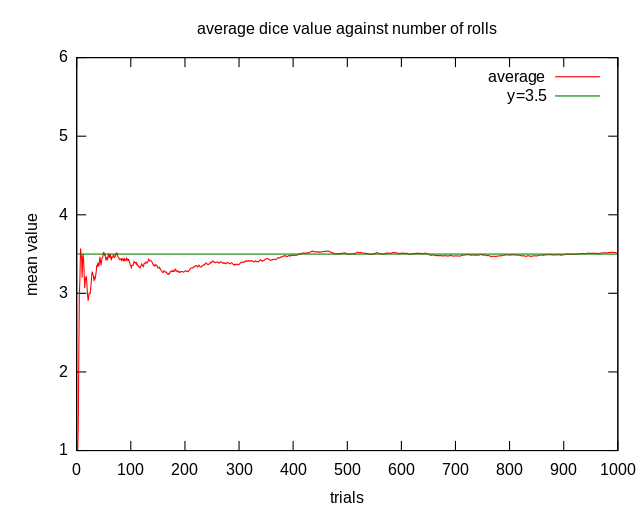
\includegraphics[width=0.6\textwidth]{c3.dashu.01.png}
    \end{figure}
  \end{block}
\end{frame}

\begin{frame}
  \frametitle{大数定律 | 引言}
  \begin{block}{中心极限定理}
中心极限定理说明,大量相互独立的随机变量,其均值的分布以正态分布为极限。这组定理是数理统计学和误差分析的理论基础,指出了大量随机变量之和近似服从正态分布的条件。
  \vspace{-1em}
  \begin{figure}
    \centering
    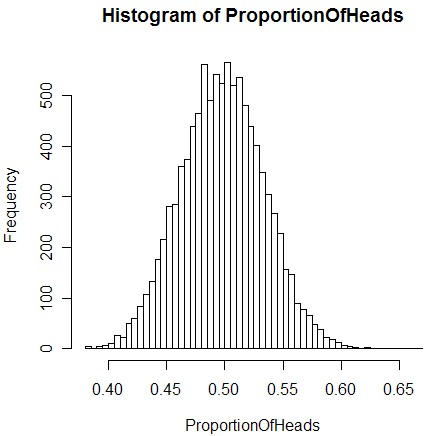
\includegraphics[width=0.45\textwidth]{c3.zhongxin.01.png}
  \end{figure}
  \end{block}
\end{frame}

\begin{frame}
  \frametitle{大数定律 | 引言}
  \begin{block}{抽奖}
    \begin{itemize}
      \item 每100人中有一人中奖
      \item 中奖概率为1\%
    \end{itemize}
    \vspace{-1em}
    \begin{figure}
      \centering
      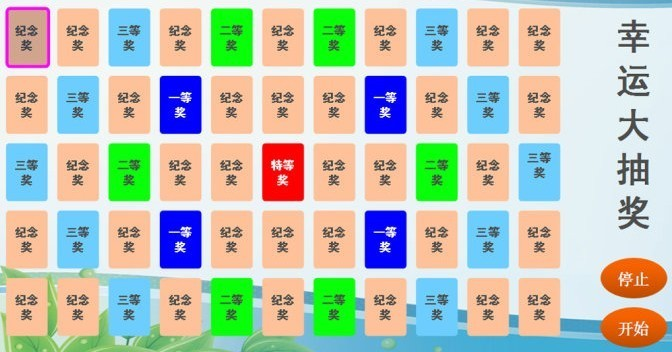
\includegraphics[width=0.8\textwidth]{c3.chance.01.jpg}
    \end{figure}
  \end{block}
\end{frame}

\subsection{案例}
\begin{frame}
  \frametitle{大数定律 | 案例 | 引言}
  \begin{block}{建议}
    在被告知某个调查的结果时,你需要做的就是反问一句:“为了得出这个结论,你调查了多少名被访者?”
  \end{block}
  \pause \pause \pause \pause
  \begin{block}{解析}
    \begin{itemize}
      \item 有偏抽样:采用严重有偏的样本几乎能够产生任何人需要的任何结果。
      \item 正确的随机样本也可以达到上述效果:
        \begin{itemize}
          \item 只要样本容量足够小(大数定律)
          \item 或者尝试足够多的次数(中心极限定理)
        \end{itemize}
    \end{itemize}
  \end{block}
\end{frame}

\begin{frame}
  \frametitle{大数定律 | 案例 | 抛硬币}
  \begin{block}{小样本}
    给定一个足够小的样本,怎样才能完全依靠机遇形成毫无指导性的结论呢?(几乎不费劲!)
  \end{block}
  \begin{figure}
    \centering
    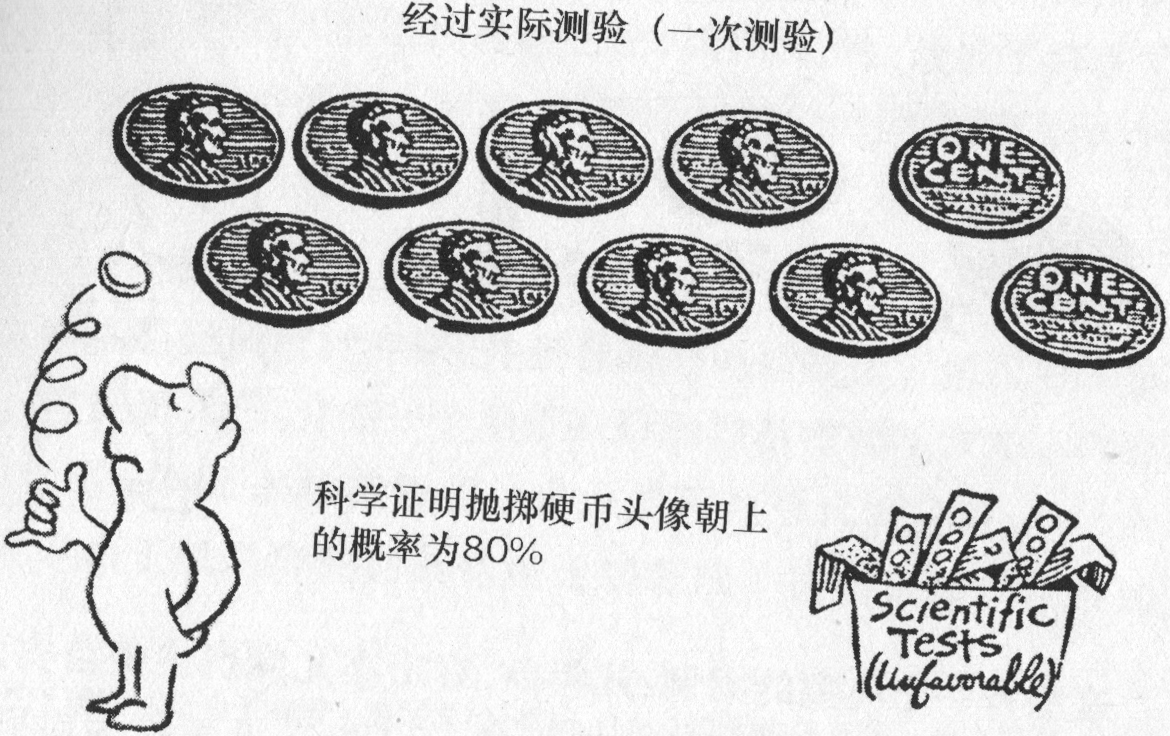
\includegraphics[width=0.8\textwidth]{c3.coin.01.png}
  \end{figure}
\end{frame}

\begin{frame}
  \frametitle{大数定律 | 案例 | 减少蛀牙的牙膏}
  \begin{block}{报道}
    “用户反映使用多克斯(Doakes)牌牙膏将使蛀牙减少23\%。”(大字标题)
  \end{block}
  \pause
  \begin{block}{谁说的?}
    结论出自一家信誉良好的“独立”实验室,并且还经过了注册会计师的证实。
  \end{block}
  \pause
  \begin{block}{经验}
    一种牙膏很难比其他牙膏好。
  \end{block}
  \pause
  \begin{block}{猜想}
    说谎?把戏!
  \end{block}
\end{frame}

\begin{frame}
  \frametitle{大数定律 | 案例 | 减少蛀牙的牙膏}
  \begin{block}{把戏}
    不充分的样本——统计角度的不充分。
    被测试的用户仅由12人组成。(小字文字)
  \end{block}
  \pause
  \begin{block}{类似案例}
    \begin{itemize}
      \item 实验室结论基于6个案例
      \item 实际效果因人而异
      \item 效果经过3D模拟,仅供参考
    \end{itemize}
  \end{block}
  \pause
  \begin{block}{思考}
    多克斯公司是怎样轻易地获得一个不存在漏洞并经得起检验的标题?
  \end{block}
\end{frame}

\begin{frame}
  \frametitle{大数定律 | 案例 | 减少蛀牙的牙膏}
  \begin{block}{实验}
    \begin{enumerate}
      \item 让规模不大的一组人持续记录6个月的蛀牙数,接着使用多克斯牙膏。
      \item 之后一定会发生以下的其中一种结果:蛀牙明前增多,蛀牙明显减少,或者蛀牙数量无显著变化。
      \item 如果是第一或者第三种结果,多克斯公司编档保存好(藏好甚至销毁),然后重新实验。
      \item 由于机遇的作用,迟早有一组被测试者将证明很好的效果,足以好到作为标题甚至引发一场广告战。
      \item 事实上,不管实验者使用的是多克斯牙膏,还是继续使用原来的品牌(甚至不使用牙膏),上述结果都会发生。
    \end{enumerate}
  \end{block}
  \pause
  \vspace{-0.5em}
  \begin{block}{总结}
    任何由于机遇产生的差异,在大样本的使用中都是微不足道的,不足以作为广告标题。
  \end{block}
\end{frame}

\begin{frame}
  \frametitle{大数定律 | 案例 | 总结}
  \begin{block}{大样本}
    只有在进行了足够多次的实验后,平均数定律才是一种有用的描述,并可用来预测。
  \end{block}
  \pause
  \begin{block}{多大?}
    多少才算够呢?这又是个棘手的问题。它取决于其他的因素,即你采用抽样方式所研究的总体容量有多大、变动程度有多大。\\
    \vspace{0.5em}
    值得一提的是,有时样本的规模与看上去的并不一致。
  \end{block}
\end{frame}

\begin{frame}
  \frametitle{大数定律 | 案例 | 小儿麻痹症疫苗实验}
  \begin{block}{“大规模”的医学实验}
    \begin{itemize}
      \item 一个社区中有450名儿童接种了疫苗,而680名儿童作为对照组没有接种疫苗。
      \item 该区域感染流行病后,在接种疫苗的儿童中,所有人都没有患上小儿麻痹症;对照组的儿童也没有发生。
    \end{itemize}
  \end{block}
  \pause \pause \pause \pause
  \begin{block}{疫苗无效?}
    \begin{itemize}
      \item 一般情况下,这种规模的小组预计只会产生2名患者。
      \item 在设计实验时,实验人员忽略了或者没能真正了解到该病的低发生率。因此,实验从一开始便注定是毫无意义的。
    \end{itemize}
  \end{block}
\end{frame}

\begin{frame}
  \frametitle{大数定律 | 案例 | 沙克疫苗}
  \begin{block}{大样本}
    我们要如何辨别,是疫苗还是概率的效果?答案是,需要有一大批的受试者。
  \end{block}
  \pause
  \begin{block}{沙克疫苗(小儿麻痹症疫苗)}
    在1950年代中期,注射沙克疫苗试验观察的孩童有将近200万,他们被分成两组。因为分配到控制组或只是因为拒绝参加而没有施打疫苗的儿童,有1388785人。其中,有609人之后患了小儿麻痹症,罹患率大约是每2280人中有一人。而接受疫苗的有接近50万人,其罹患率大约是每6000人中有一人。
  \end{block}
  \pause
  \begin{block}{结论}
    在这么庞大的人数中,数字的差异已经相当显著,研究团队可以确信,他们已经超越了概率。即使如此,他们还是详细检验,以确定各组的感染率并没有因为概率而造成差异。
  \end{block}
\end{frame}

\begin{frame}
  \frametitle{中心极限定理 | 案例 | 引言}
  \begin{block}{概率}
    同时发生的多起罕见事故不一定是由同一个原因所造成的。\\
    \vspace{0.5em}
    生活中的异常数字,包括罹病概率等,也不一定是由外力或单一原因所引起的,而是有冷酷无情的规则,能够合理、悲哀地被预见。\\
    \vspace{0.5em}
大家都知道事物有时会成群出现(向来都是如此),但对于干扰我们日常生活的事,大家却习惯性地将这种必然性,贴上“神秘”的标签,把正常现象称为“可疑”,把可预期的结果,叫做“反常”。\\
    \vspace{0.5em}
    在大多数情况下,事情本是概率造成的结果,但我们很难说服自己去相信这个事实。
  \end{block}
\end{frame}

\begin{frame}
  \frametitle{中心极限定理 | 案例 | 集群}
  \begin{block}{集群}
    一般人容易低估集群的大小及发生概率。
  \end{block}
  \pause
  \begin{block}{实验}
    \begin{itemize}
      \item 洗牌:拿掉大小王,洗好一副52张的扑克牌。从最上方的牌开始,一一将你手上的牌,分成红、黑色两堆。猜猜看,同一个颜色的牌,最多会连续出现几次?
      \item 掷硬币:猜猜一个硬币连续掷30次的结果。
    \end{itemize}
  \end{block}
  \pause \pause \pause \pause
  \begin{block}{结果}
    \begin{itemize}
      \item 大多数的人会猜三次。事实是,很可能会有一次连续分到五六张相同颜色的牌。
      \item 很多人觉得同一面差不多会连续出现三次。事实上,同一面连续出现五次的概率是很常见的。
    \end{itemize}
  \end{block}
\end{frame}

\begin{frame}
  \frametitle{中心极限定理 | 案例 | 集群(一千万次模拟)}
  \vspace{-1em}
\begin{table}[]
\centering
\resizebox{\textwidth}{!}{%
\begin{tabular}{crcrc}
\hline
\multicolumn{1}{l}{连续同} & \multicolumn{2}{c}{52张扑克牌} & \multicolumn{2}{c}{30枚硬币} \\
\multicolumn{1}{l}{颜色/面} & \multicolumn{1}{c}{次数} & 百分比 & \multicolumn{1}{c}{次数} & 百分比 \\ \hline
... & ... & ... & ... & ... \\
% 1 & 134998483 & 1349 & 80003557 & 800 \\
% 2 & 66235606 & 662 & 38745994 & 387 \\
3 & 32504441 & 325 & 18751126 & 187 \\
4 & 15947069 & 159 & 9059847 & 90 \\
5 & 7812504 & 78 & 4374944 & 43 \\
6 & 3828248 & 38 & 2108988 & 21 \\
7 & 1874140 & 18 & 1014742 & 10 \\
% 8 & 916608 & 9 & 489684 & 4 \\
% 9 & 447796 & 4 & 234683 & 2 \\
% 10 & 219978 & 2 & 112668 & 1 \\
... & ... & ... & ... & ... \\
% 27 & 0 & 0 & 1 & 0 \\
% 28 & 2 & 0 & 0 & 0 \\
29 & 1 & 0 & 0 & 0 \\
30 & 1 & 0 & 0 & 0 \\ \hline
\end{tabular}%
}
\end{table}
\end{frame}

\begin{frame}
  \frametitle{中心极限定理 | 案例 | 癌症村}
  \begin{figure}
    \centering
    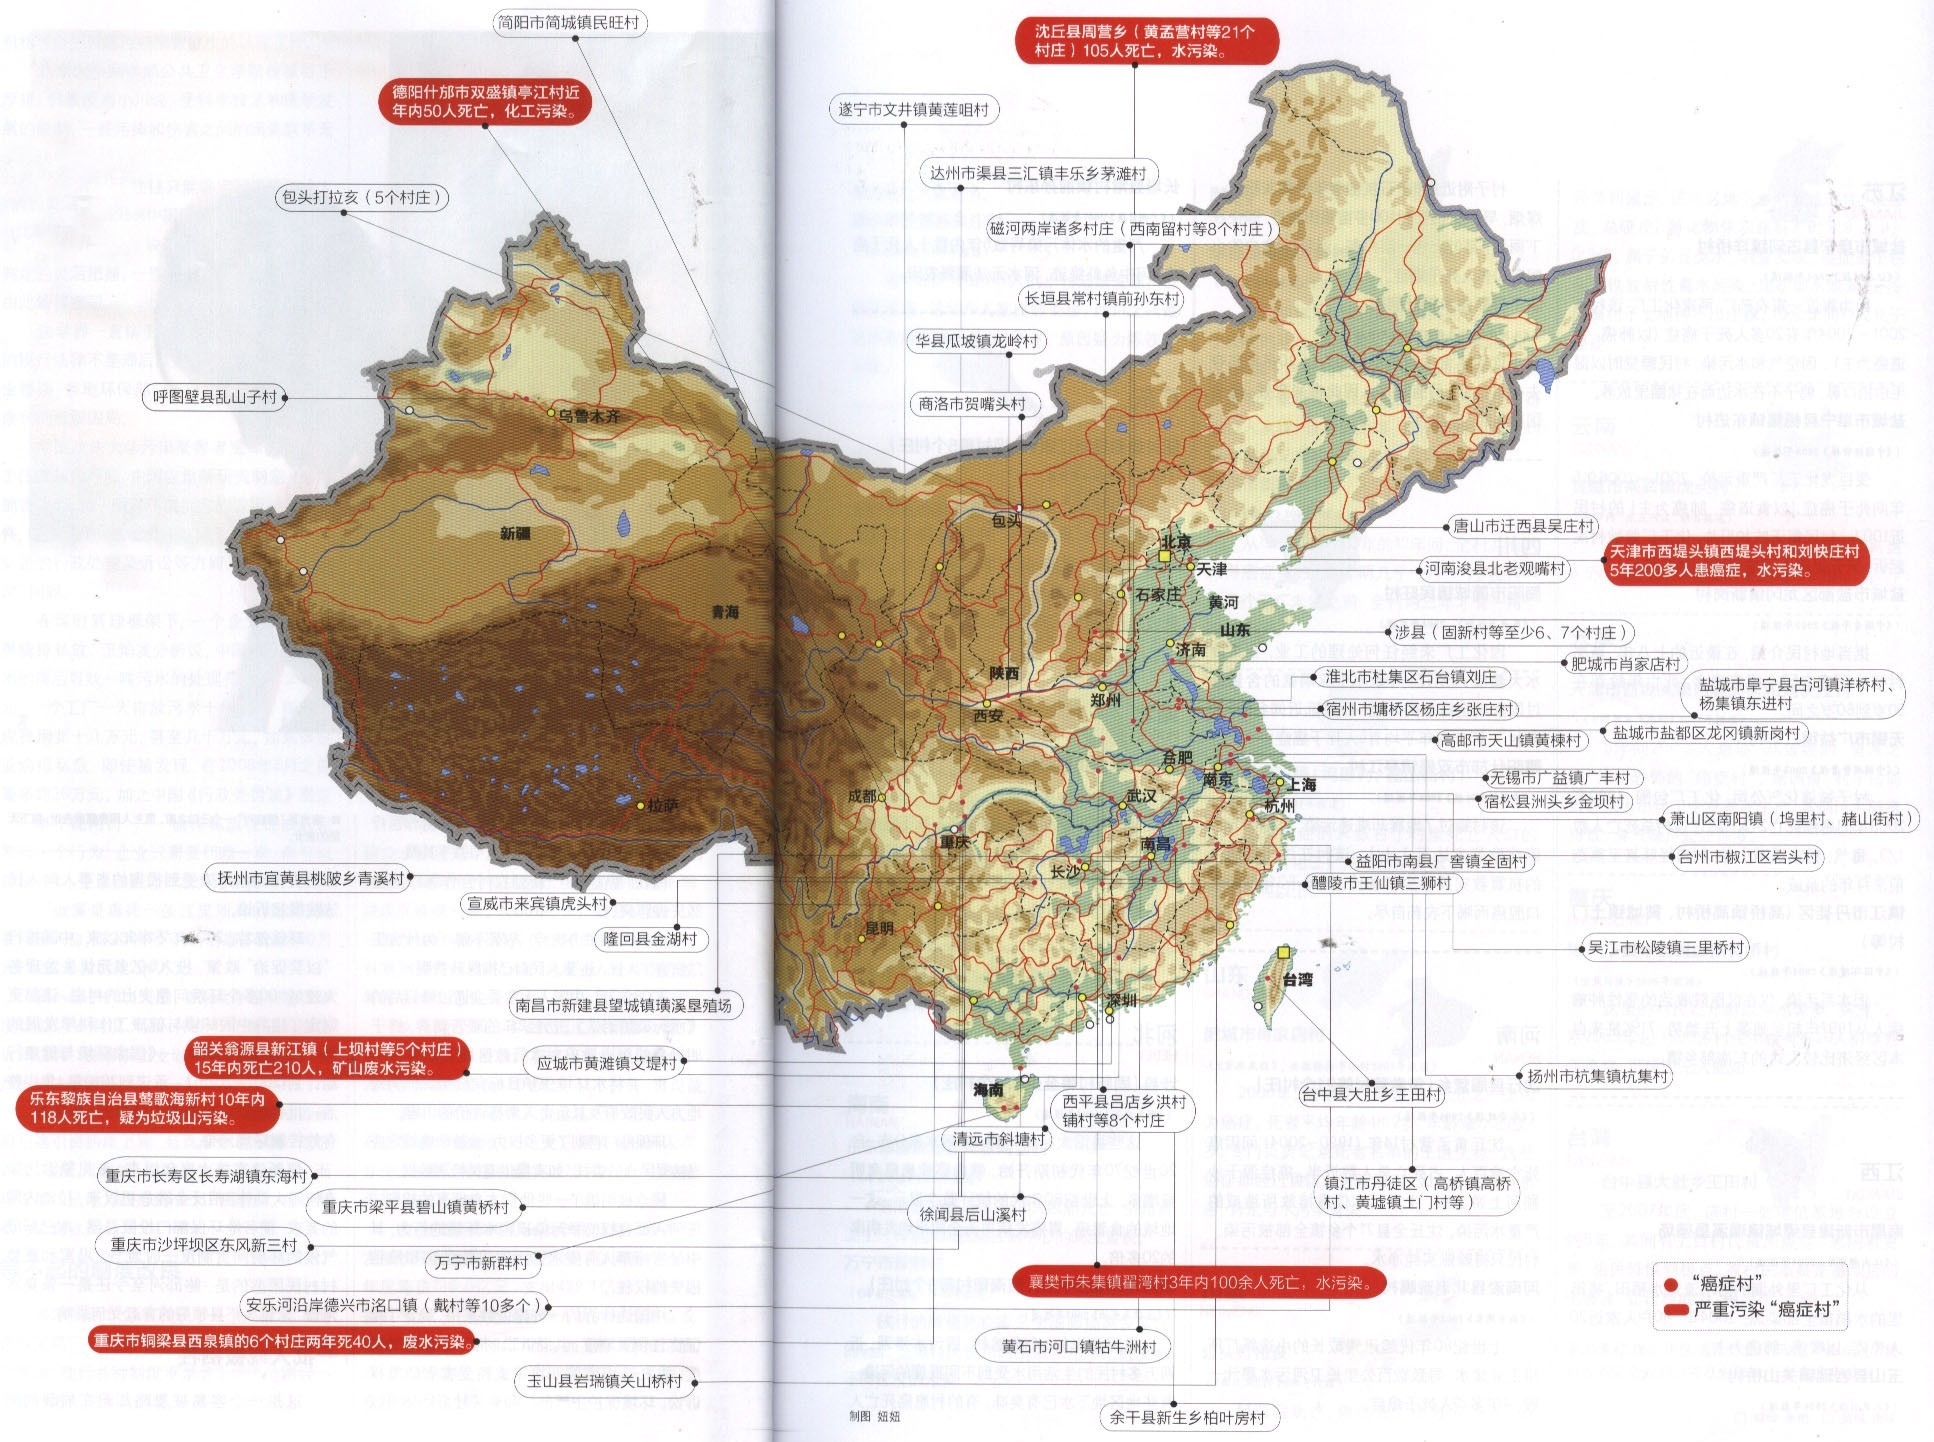
\includegraphics[width=0.85\textwidth]{c3.cancer.02.jpg}
  \end{figure}
\end{frame}

\begin{frame}
  \frametitle{中心极限定理 | 案例 | 癌症村}
  \begin{figure}
    \centering
    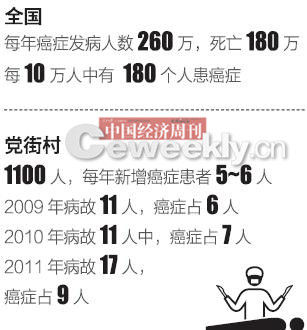
\includegraphics[width=0.6\textwidth]{c3.cancer.01.jpg}
  \end{figure}
\end{frame}

\section{均值回归}
\subsection{引言}
\begin{frame}
  \frametitle{均值回归 | 引言}
  \begin{block}{均值回归}
    均值回归是指股票价格、房产价格等社会现象、自然现象(气温、降水),无论高于或低于价值中枢(或均值)都会以很高的概率向价值中枢回归的趋势。\\
    \vspace{1em}
根据这个理论,一种上涨或者下跌的趋势不管其延续的时间多长都不能永远持续下去,最终均值回归的规律一定会出现:涨得太多了,就会向平均值移动下跌;跌得太多了,就会向平均值移动上升。
  \end{block}
\end{frame}

\begin{frame}
  \frametitle{均值回归 | 引言}
  \begin{block}{经验}
    在其他条件完全相等的情况下,如果最近的数字比平常水平高,你可以预期接下来的数字有可能会下降,而不是上升。
  \end{block}
  \pause
  \begin{block}{回归至平均数(regression to the mean)}
    当一个数字靠近达到顶点或最低点时,接下来便可能朝向平均值移动。
  \end{block}
  \pause
  \begin{block}{现象}
    那些反复被拿出来歌功颂德的极少数有效政策,很多都是因为概率或好运而成功达成目标,并非他们所说的,是因为施政正确而造成的差异。
  \end{block}
\end{frame}

\subsection{案例}
\begin{frame}
  \frametitle{均值回归 | 案例 | 身高}
  \begin{figure}
    \centering
    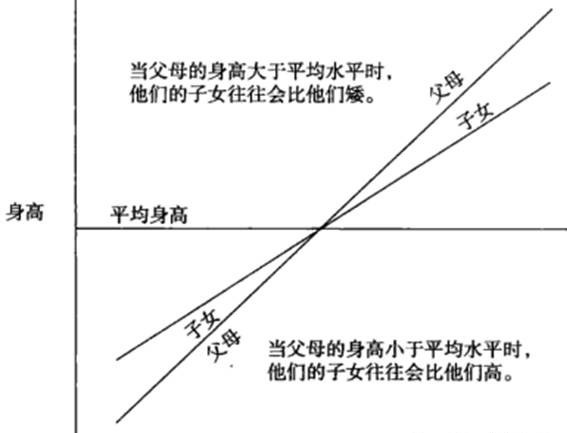
\includegraphics[width=0.8\textwidth]{c3.height.01.jpg}
  \end{figure}
\end{frame}

\begin{frame}
  \frametitle{均值回归 | 案例 | 测速照相机}
  \begin{block}{测速照相机}
    安装测速照相机,车祸究竟是增加还是减少?
    一个为期两年的独立实验计划,允许8个地区将收到的超速罚款投资设置更多的测速照相机。
  \end{block}
  \begin{figure}
    \centering
    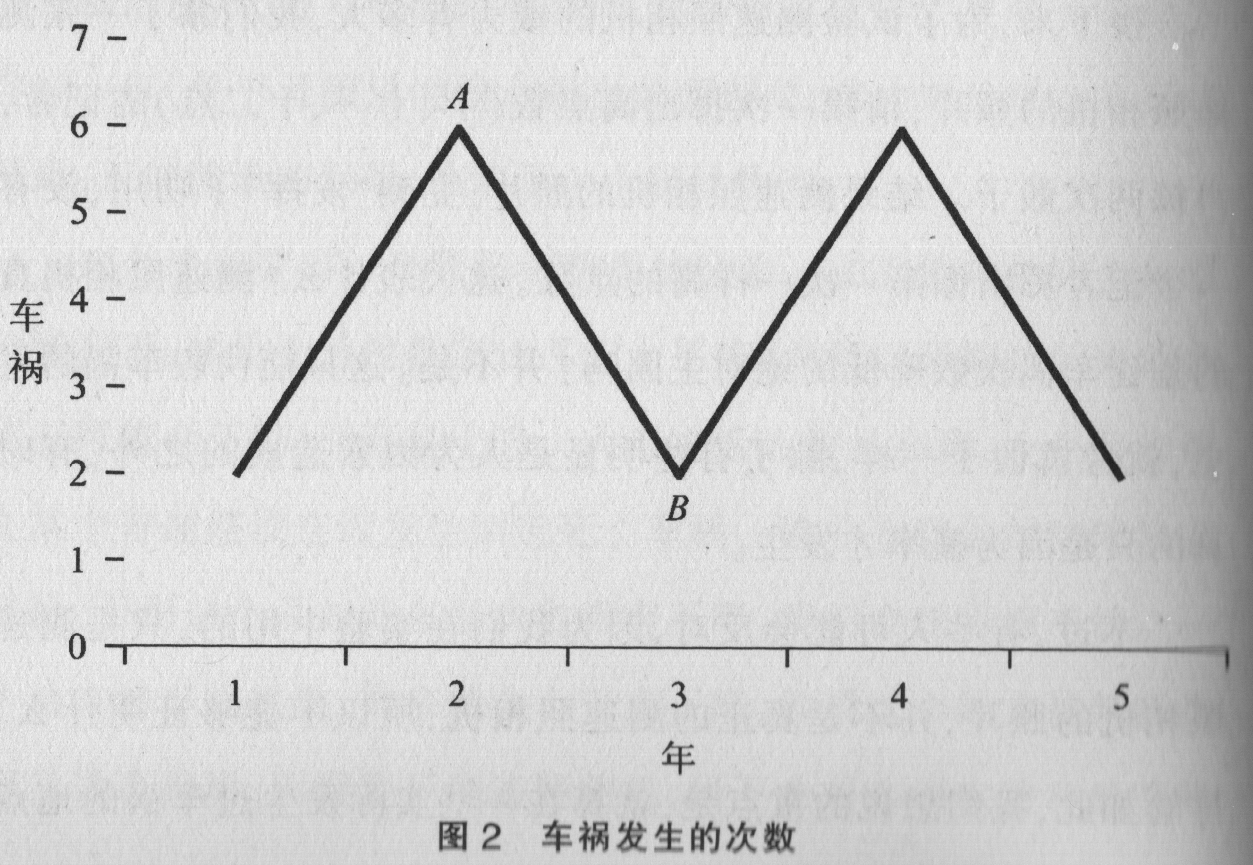
\includegraphics[width=0.7\textwidth]{c3.camera.01.png}
  \end{figure}
\end{frame}

\begin{frame}
  \frametitle{均值回归 | 案例 | 测速照相机}
  \begin{block}{结论}
    \begin{itemize}
      \item 在所有安装测速照相机的地点所减少的死伤车祸中,约有60\%被归为回归至平均数的现象。
      \item 有18\%则被归为所谓的“趋势”,即全国车祸次数普遍下降,包括没有安装测速照相机的地方,而原因可能和路面、汽车安全性能等的改善有关。
      \item 其余的20\%左右,则明显是测速照相机本身的功效(仍有点争议)。
    \end{itemize}
  \end{block}
\end{frame}

\section{误差}
\subsection{引言}
\begin{frame}
  \frametitle{误差 | 引言}
  \begin{block}{误差}
    误差(errors)是实验科学术语。指测量结果偏离真值的程度。\\
    \vspace{0.3em}
对任何一个物理量进行的测量都不可能得出一个绝对准确的数值,即使使用测量技术所能达到的最完善的方法,测出的数值也和真实值存在差异,这种测量值和真实值的差异称为误差。\\
\vspace{0.3em}
数值计算分为绝对误差和相对误差。也可以根据误差来源分为系统误差、随机误差和毛误差。
  \end{block}
  \pause
  \begin{block}{随机误差}
    随机误差(Random error),无法控制的变因,会使得测量值产生随机分布的误差。它服从统计学上所谓的“正态分布”或称“高斯分布”,它是不可消除的,在这个意义上,测量对象的真值是永远不可知的,只能通过多次测量获得的均值尽量逼近。\\
    \vspace{0.3em}
    系统误差以相同的方式影响所有测量值,将它们推向同一个方向;随机误差,则随着不同次的测量而变化,有时候向上或向下。
  \end{block}
\end{frame}

\begin{frame}
  \frametitle{误差 | 引言}
  \begin{figure}
    \centering
    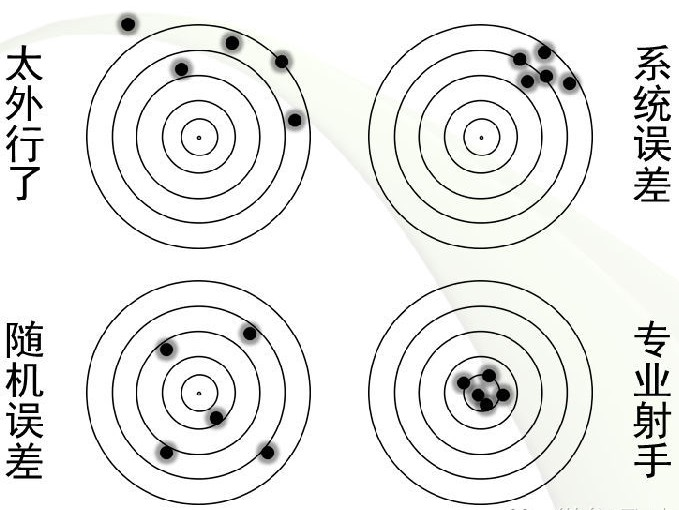
\includegraphics[width=0.8\textwidth]{c3.error.03.jpg}
  \end{figure}
\end{frame}

\begin{frame}
  \frametitle{误差 | 引言}
  \begin{block}{怎么办?}
    如何避免被不科学的结论所愚弄呢?是否每个人都必须成为自己的统计专家,并亲自研究原始数据?
  \end{block}
  \pause
  \begin{block}{显著性检验}
    一种反映检验数据以多大的可能性代表实际结论、而不是代表由于机遇产生的其他结论的方法。\\
    \vspace{0.3em}
    显著性程度通常简单地用概率来表示,就像普查局以19/20的概率保证他们的结果是正确的。\\
    \vspace{0.3em}
大多数情况下,5\%的显著性水平已经足够,但是如果有更高的要求,就需要1\%的显著性水平,这意味着以99\%的概率保证该结果是真实的,任何类似的事情“在实践上几乎是确定”的。
  \end{block}
\end{frame}

\begin{frame}
  \frametitle{误差 | 引言}
  \begin{block}{显著性差异}
显著性差异(p),是统计学上对数据差异性的评价。当数据之间具有了显著性差异,就说明参与比对的数据不是来自于同一总体(Population),而是来自于具有差异的两个不同总体。\\
\vspace{0.3em}
  这种差异可能因参与比对的数据是来自不同实验对象;也可能来自于实验处理对实验对象造成了根本性状改变,因而前测后测的数据会有显著性差异。
  \end{block}
  \pause
  \begin{block}{表述}
    显著性差异是一种有量度的或然性评价。通常情况下,实验结果达到0.05或0.01水平,才可以说数据之间具备了显著性差异。通常用于假设检验,检验假设和实验结果是否一致。\\
    \vspace{0.3em}
我们说A、B两数据在0.05水平上具备显著性差异,这是说两组数据具备显著性差异的可能性为95\%。两个数据所代表的样本还有5\%的可能性是没有差异的。这5\%的差异是由于随机误差造成的。\\
  \end{block}
\end{frame}

\begin{frame}
  \frametitle{误差 | 引言}
  \begin{figure}
    \centering
    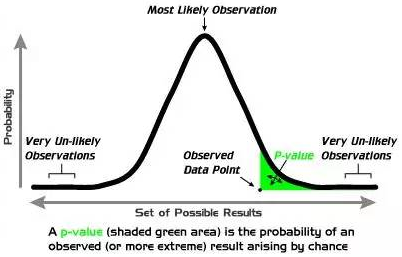
\includegraphics[width=0.5\textwidth]{c3.p.01.png}\\
    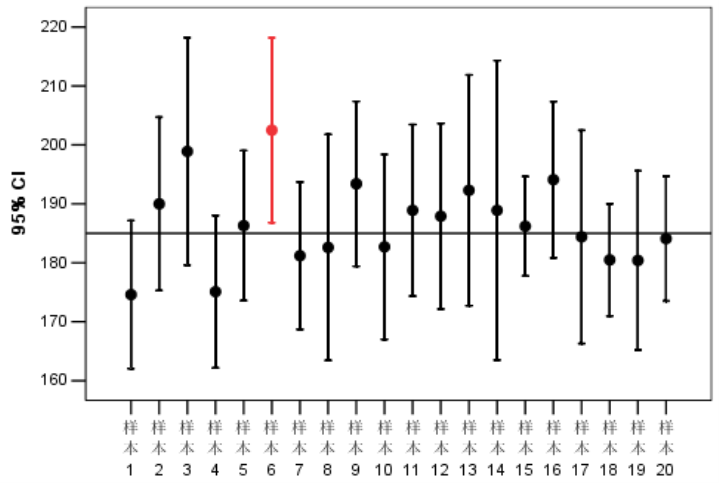
\includegraphics[width=0.5\textwidth]{c3.p.02.png}
  \end{figure}
\end{frame}

\begin{frame}
  \frametitle{误差 | 案例 | 总结}
  \begin{block}{误差}
    重要的不是数字的对错,因为它们往往会出错,重要的是它们是否错到会误导我们的判断。\\
    \vspace{0.3em}
统计学上的标准做法是:虽然我们可能连某个数字到底是太高或太低都不知道,但大家会先预估数字出错的程度。把估计值加上可能的误差大小是预防数字出错的最好办法,而一般的惯例是,先表明估计值会落在哪个范围之内,此范围正确的概率为95\%——称为置信区间(confidence interval)。就算有了95\%的置信区间,仍旧有5\%的概率会出错。
  \end{block}
  \pause
  \begin{block}{注意}
在看一个数字时,你应记得问:“它们有这么精确吗?”而答案往往是:它们可能无法、也不是这么精确也不是这么精确,但新闻报道为了力求简洁,把所有的怀疑都扫到地毯下藏了起来。如果新闻报道中,有某个地方忽然蹦出不确定性,那倒是值得我们好好了解一下,它想要表达什么。
  \end{block}
\end{frame}

\subsection{案例}
\begin{frame}
  \frametitle{误差 | 案例 | 智力测试}
  \begin{block}{智力测试}
    \begin{itemize}
      \item 智商的平均数是100,即100意味着“正常”。
      \item 琳达的智商是101,彼得只有98。
    \end{itemize}
  \end{block}
  \pause
  \begin{block}{结论}
    琳达是比较聪明的孩子,而且她的智商高于平均水平,彼得则低于平均水平。
  \end{block}
\end{frame}

\begin{frame}
  \frametitle{误差 | 案例 | 智力测试}
  \begin{block}{智力测验 vs. 智商}
    无论智力测验测试的是什么,它与我们通常意义上的智商都不是一码事。它忽略了类似领导才能、创造性想象力等十分重要的素质;没有考虑到社交判断力以及音乐、艺术等方面的才能;无法测试出诸如勤劳、情感平衡等重要的人格品质。
  \end{block}
  \pause
  \begin{block}{统计误差}
    智力测试只是智力水平的一个抽样。与其他抽样结果一样,代表智力水平的智商值也具有统计误差,这个误差将用来衡量该数值的准确度或可信度。
  \end{block}
\end{frame}

\begin{frame}
  \frametitle{误差 | 案例 | 智力测试}
  \begin{block}{误差}
    可能误差和标准误差可以定量地衡量你的样本以多大的精度代表总体。
  \end{block}
  \pause
  \begin{block}{智力测验}
    假设智力测验的可能误差为3\%。这与智力测验的好坏无关,只是反映了测验与它所能测试的内容具有怎样的一致性。
  \end{block}
  \pause
  \begin{block}{智商}
    琳达的智商更全面的表达是101$\pm$3,彼得的智商则是98$\pm$3。
  \end{block}
  \pause
  \begin{block}{结论}
    正常的智商不应该只是100这样一个数值,而应是诸如90~100的一个范围。将处于这个范围的孩子与低于或高于此范围的孩子进行比较时会得出一些有用的结论。
  \end{block}
\end{frame}

\begin{frame}
  \frametitle{误差 | 案例 | 智力测试 | 总结}
  \begin{block}{总结}
    \begin{itemize}
      \item 对待智力测验以及许多其他类似的抽样结果应注意它的范围。
      \item 必须在脑中牢记这个加减符号,即使(特别是当)它没有明确给出。
      \item 比较相差不大的两个数据毫无意义。
      \item 在所有抽样研究中都有误差,忽略这些误差将导致一些愚蠢的举动。
    \end{itemize}
  \end{block}
\end{frame}

\begin{frame}
  \frametitle{误差 | 案例 | 读者调查}
  \begin{block}{女性杂志的编辑的读者调查}
    对于一篇有40\%男性读者喜爱的文章与另一篇只有35\%男性读者喜爱的文章,他们会刊载更多类似于前者的作品。
  \end{block}
  \pause \pause \pause \pause
  \begin{block}{解析}
    \begin{itemize}
      \item 对于杂志而言,40\%与35\%读者人数的差异是很重要的,但抽样调查形成的差别却并不一定是真实的。
      \item 出于成本的考虑,读者人数调查的实际样本,特别是已经扣除了那些从来不读该杂志的人后,也许只有几百人。
      \item 对于一本女性杂志,样本中的男性读者会很少。当这些人又根据他们的回答:“全部读了”、“读了大部分”、“读了一部分”以及“没看”这篇文章而划分成四组后,35\%男性读者的结论也许仅仅建立在几个人基础之上。
      \item 隐藏在这个看似显著的数据背后的误差可能会很大。
    \end{itemize}
  \end{block}
\end{frame}

\begin{frame}
  \frametitle{误差 | 案例 | 老黄金香烟}
  \begin{block}{实验}
    \begin{itemize}
      \item 实验:《读者文摘》编辑聘请一些实验室人员对不同品牌香烟的烟雾展开分析。
      \item 结果:列出每种品牌香烟的烟雾中尼古丁以及其他有害物质的含量。
      \item 结论:所有品牌的香烟是一样的,无论你吸的是什么牌子的香烟,不会有任何差异。
    \end{itemize}
  \end{block}
  \vspace{-0.3em}
  \pause
  \begin{block}{报道}
    \begin{itemize}
      \item 发现:在一长串具有相同有害物质的品牌名单上,总有一个排在最后,这就是“老黄金(Old Gold)”牌香烟。
      \item 报道:由一家国家级杂志主持的实验证明“老黄金”牌香烟在不良物质,以及尼古丁含量方面“排在最后”。
      \item 省略:任何关于各个品牌的差异并不显著的文字甚至是暗示都被省略了。
    \end{itemize}
  \end{block}
\end{frame}

\section{偷梁换柱}
\subsection{引言}
\begin{frame}
  \frametitle{偷梁换柱 | 引言}
  \begin{block}{不完全匹配的资料}
    \begin{itemize}
      \item 如果你想证明某事,却发现没有能力办到,那么就试着解释其他相关事情,并假装它们是一回事。
      \item 在统计资料与人类思维冲撞所引起的耀眼光芒中,几乎没有人会发现它们的区别。
      \item 不完全匹配的资料是一种保证你处在有利位置上的武器,而且屡试不爽。
      \item 一般的做法是将看上去极像、而完全不同的两件事混淆在一起。
    \end{itemize}
  \end{block}
\end{frame}

\subsection{案例}
\begin{frame}
  \frametitle{偷梁换柱 | 案例 | 感冒药}
  \begin{block}{报道}
    你无法证明你的秘方能够治疗感冒,但你却可以在报纸上刊登一篇得到保证的实验室报告,“在11秒内仅仅半盎司的该药剂量就杀死了试管中31108个细菌”。(佐证:著名实验室、报告全文复印件、 穿白大褂医生的照片)
  \end{block}
  \pause \pause \pause \pause
  \begin{block}{没有提及的小把戏}
    \begin{itemize}
      \item 在试管中很有效的抗菌剂,在人的喉咙里就不会发挥作用。
      \item 为了防止该药灼烧喉咙要按照说明书进行稀释。
      \item 不要报道杀死了哪些细菌。(谁会知道哪种细菌引起了感冒?说不定感冒根本就与细菌无关。)
    \end{itemize}
  \end{block}
\end{frame}

\begin{frame}
  \frametitle{偷梁换柱 | 案例 | 喉宝牌香烟}
  \begin{block}{报道}
    对著名医生组成的大样本调查结果显示:27\%的医生抽的是喉宝(Throaties)这个牌子的香烟,该比例高于其他所有品牌。
  \end{block}
  \begin{figure}
    \centering
    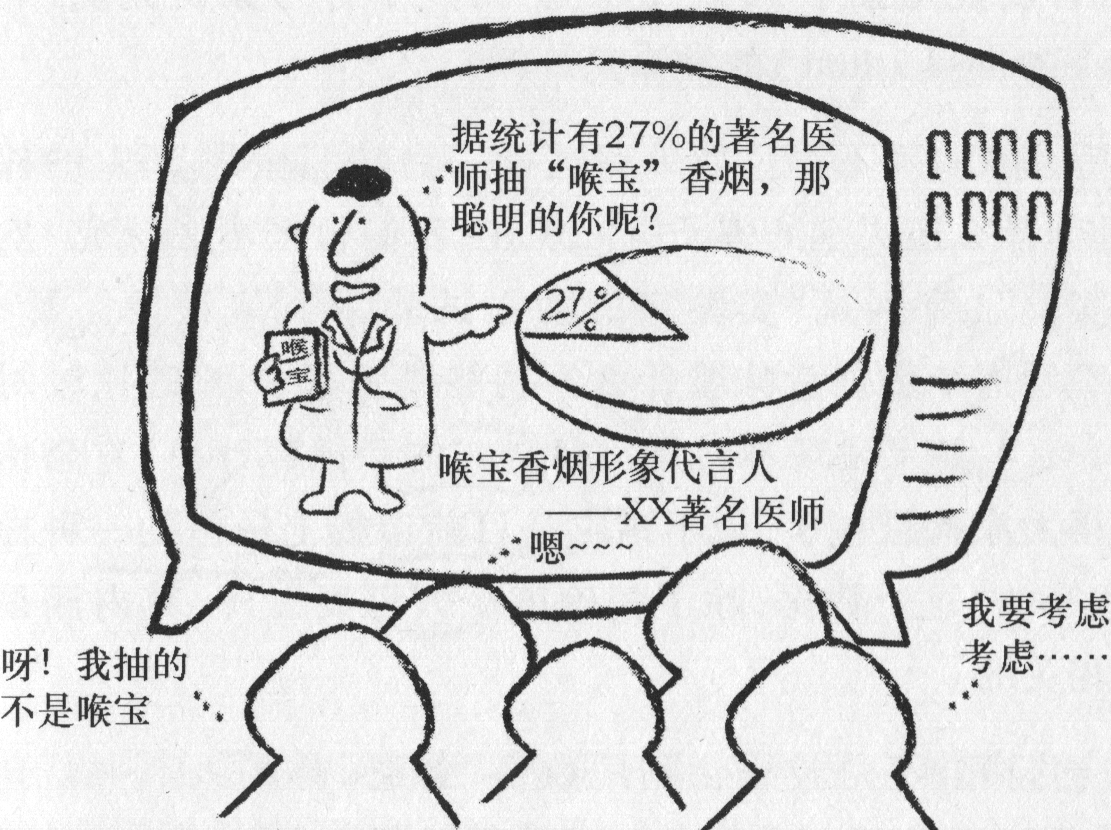
\includegraphics[width=0.7\textwidth]{c3.cigar.01.png}
  \end{figure}
\end{frame}

\begin{frame}
  \frametitle{偷梁换柱 | 案例 | 喉宝牌香烟}
  \begin{block}{解析}
    \begin{itemize}
      \item 是否拥有了人们对医务职业的尊敬,医生就会比其他人掌握更多关于香烟品牌的信息?
      \item 是否他们会有内部消息帮助他们选择危害性更低的品牌?
    \end{itemize}
  \end{block}
  \pause
  \begin{block}{结论}
    对于这种不相关的数据,唯一的回答是:“那又如何?”
  \end{block}
\end{frame}

\begin{frame}
  \frametitle{偷梁换柱 | 案例 | 病人的等待时间}
  \begin{block}{病人的等待时间}
    (英国)政府当局为医疗服务设定了一个新目标,依据现行的规定,病人等待手术的时间,不得超过6个月,诊所医生将病人转诊之后,他们获得医治的时间,不得超过13周。
    政府当局大肆吹嘘,说该政策已经使得等待治疗的时间缩短(“等待手术的时间……比以往都短”)。
  \end{block}
  \pause \pause \pause \pause
  \begin{block}{解析}
    \begin{itemize}
      \item 虽然最长的等待治疗时间的确大幅缩短,但这些病人只占总等待人数的极小比例。
      \item 如果要说政府已经成功缩短等最久病人的等待时间,也相当合理,但不应扩大为“等待时间减少”。
    \end{itemize}
  \end{block}
\end{frame}

\begin{frame}
  \frametitle{偷梁换柱 | 案例 | 自杀率}
  \begin{block}{青少年具有较多自杀倾向}
    一家德国报纸文章“老年时会变得更幸福”分析论证了下面的结果:在20岁以下的青少年中,自杀在所有死亡中所占的比例最大,共计25\%。而30~40岁的人自杀率占到10\%,超过70岁的老年人自杀率不足2\%。“年龄越大,决定自杀的比率就越低”。
  \end{block}
  \pause \pause \pause \pause
  \begin{block}{解析}
    事实正好相反。随着年龄的不断增长,自杀率在上升,20岁以下的青少年自杀率不足$1/10^5$,70岁以上老年人的自杀率则几乎达到$50/10^5$。我们的年龄越大,就越容易做出决定,自愿结束自己的生命,这种现象存在于各个国家的各个时期。\\
    \vspace{0.3em}
自杀在青少年那里的确起着一个非常显著的作用,其原因主要是青少年一般来说很少自然死亡。换句话说,在青少年年龄段,事故、谋杀和自杀几乎是主要的死亡原因,而自杀在各类死亡中所占的比例又比较高。
  \end{block}
\end{frame}

\begin{frame}
  \frametitle{偷梁换柱 | 案例 | 交通安全}
  \begin{block}{报道}
    \begin{itemize}
      \item 天气晴朗时驾车比有雾时更危险。
      \item 去年因飞机失事造成的死亡人数比1910年多,这是否意味着乘坐现代化的飞机反而更危险?
      \item 在最近的一年中,火车交通的死亡人数为4712人。
    \end{itemize}
  \end{block}
  \pause \pause \pause \pause
  \begin{block}{解析}
    \begin{itemize}
      \item 因为晴天比雾天多,所以天气晴朗时会有更多的交通意外发生。
      \item 现在选择飞机作为交通工具的人已经是以前的几百倍了。
      \item 4712人中仅有132人是火车上的乘客,其余都是无票偷乘或者在十字路口相撞的人。(必须将这个数据与总乘客、里程数相结合才有意义。)
    \end{itemize}
  \end{block}
\end{frame}

\section{比较}
\subsection{引言}
\begin{frame}
  \frametitle{比较 | 引言}
  \begin{block}{比较}
    比较是一种评量及判断的基本工具。但过度注重比较会落入各式各样的陷阱中,意外的或故意的都有。任何有效力的比较,都必须拿同类的事物相比。
    \vspace{-2em}
    \begin{figure}
      \centering
      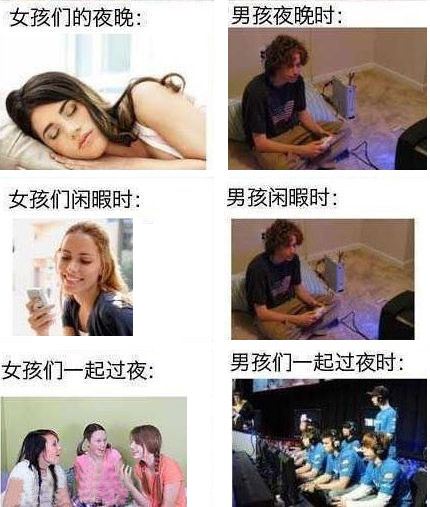
\includegraphics[width=0.4\textwidth]{c3.compare.01.jpg}
    \end{figure}
  \end{block}
\end{frame}

\subsection{案例}
\begin{frame}
  \frametitle{比较 | 案例 | 榨汁机}
  \begin{block}{报道}
    “经过实验室的证明”该榨汁机的“榨汁功能增强了26\%”,并且“得到了好管家研究院的推荐”。
  \end{block}
  \pause \pause \pause \pause
  \begin{block}{解析}
    功能增强了26\%的比较对象是什么?(如果不过是一台老式的手摇榨汁机……)
  \end{block}
  \pause
  \begin{block}{类似}
    \begin{itemize}
      \item 和某知名品牌相比……
      \item 和同类产品相比……
    \end{itemize}
  \end{block}
\end{frame}

\begin{frame}
  \frametitle{比较 | 案例 | 电子监控器的效果}
  \begin{block}{报道}
    相较于未戴电子监控器的罪犯高达67\%左右的再犯率,在13万个戴过电子监控器的受刑人中,戴着监控器再犯的比率大约是4\%。
  \end{block}
  \pause \pause \pause \pause
  \begin{block}{解析}
    \begin{itemize}
      \item 谁与谁比?两种罪犯并非同一种人。
      \item 何时比较?4个半月 vs. 两年。
      \item 比较什么?和替代方案进行比较。
    \end{itemize}
  \end{block}
  \pause
  \begin{block}{正确的比较}
    \begin{itemize}
      \item 戴过电子监控器服刑期满以及在牢里服刑期满这两组人
      \item 目前戴着电子监控器的受刑人以及正在牢里服刑的受刑人
    \end{itemize}
  \end{block}
\end{frame}

\begin{frame}
  \frametitle{比较 | 案例 | 教师收入}
  \begin{block}{报道}
    在1942年杜威当选州长时,一些地区教师的最低年收入只有900美元;而今天,纽约州的教师享有全世界最高的收入水平。在杜威政府的建议下,在由杜威指定的委员会的表决下,立法机构于1947年从州财政盈余中拨出3200万美元直接用于提高教师收入水平,这使得纽约市教师最低收入水平提高到2500~5323美元之间。
  \end{block}
  \pause \pause \pause \pause
  \begin{block}{解析}
    这里使用了前后比较的老把戏,一些未被指明的因素加入到过程中,导致前后并不一致。实际上,900美元是该州所有乡村地区的最低收入,2500~5323仅仅是纽约市的最低收入水平。
  \end{block}
\end{frame}

\begin{frame}
  \frametitle{比较 | 案例 | 学校排名}
  \begin{block}{排名}
    学校、医院、警力、地方政府,或任何接受排名及绩效评估的单位,都应该属于相同类型,可惜通常不是如此,而且很少能够尽如人意。生活本来就是混乱复杂,差异远比预期的更多、更大、更显著,在忽略差异之前,我们得先决定,自己是否在意忽略差异所代表的妥协及不公正。
  \end{block}
  \pause
  \begin{block}{学校绩效排名制度}
    英国在1992年引进学校绩效排名制度。2007年,学校绩效排名制度经历了第三次重大的修改,让一些学校及其绩效彻底改变排名顺序。这些学校的学生考试成绩并没有明显的变化,但许多原本属于一流学校的却被打入二三流,而有些原本在边缘挣扎的学校却瞬间成为绩优学校。
  \end{block}
\end{frame}

\begin{frame}
  \frametitle{比较 | 案例 | 国际比较}
  \begin{block}{国际比较}
  假设我们都同意,在地区板球比赛得到100分代表很会运动,我们可以比出一个结果:三次被票选为年度最佳足球选手的齐达内,将会因为无法在板球比赛中拿到100分而变成运动白痴。这种比较方法很荒谬,但却是国际比较的常态。
  \end{block}
  \pause
  \begin{block}{越狱}
    芬兰的一组监狱从来没有发生过越狱事件,年复一年,都没有人逃跑。莫非他们用的方法,是全球监狱最值得效法的典范?——开放式监狱!
  \end{block}
\end{frame}

\begin{frame}
  \frametitle{比较 | 案例 | WHO的医疗体系排行}
  \begin{block}{WHO的医疗体系排行}
    英国只卑微地排名第18;最富强的美国居然排名第50。
  \end{block}
  \pause
  \begin{block}{解析}
    WHO在汇编这个排行时,所考虑的因素包括:平均寿命、婴儿死亡率、丧失自理能力后的存活年数、维护病人尊严的程度、隐私性、病人选择医疗的参与度、系统是否为“顾客导向”、保健支出的产出效能等。大多数的人会说,这些因素大部分都很重要,但哪一项最重要?是否还有其他项目遗漏了,却更重要?
  \end{block}
\end{frame}

\begin{frame}
  \frametitle{比较 | 案例 | 数学能力}
  \begin{block}{英德数学能力比较}
    孩童学数学,最重要的是要学到什么?在2006年的一项排行中,德国超前英国,但在另一项排行中,英国却超前德国。
  \end{block}
  \pause \pause \pause \pause
  \begin{block}{解析}
    \begin{itemize}
      \item 两项测验考的是不同的数学能力。(采用两套不同的测验,依据不同的标准来评量。)
      \item “数学”的定义很广,英国学生比较擅长数学技巧的实际应用,如应该如何制定一场表演的票价才能回收成本并有机会赚钱,而德国学生则比较擅长传统数学,如分数等。
    \end{itemize}
  \end{block}
\end{frame}

\begin{frame}
  \frametitle{比较 | 案例 | 婴儿死亡率}
  \begin{block}{婴儿死亡率}
    在德国西部1000名婴儿中就有19名没有存活下来,这个比例远远高于中国香港(15名)和新加坡(14名)。
  \end{block}
  \pause
  \begin{block}{疑问}
    在有选择性地列举的这些地区和国家中,一个明显的事实是,它们在医疗卫生和健康方面都比德国弱。
  \end{block}
  \pause \pause \pause \pause
  \begin{block}{解析}
    “婴儿死亡”的定义:在德国,“婴儿死亡”是指所有或者出生的婴儿,其在第一年中死亡的,当然并不包括刚一出生时就已经死亡的。
  \end{block}
\end{frame}

\section{单一数字}
\subsection{引言}
\begin{frame}
  \frametitle{单一数字 | 引言}
  \begin{block}{单一数字}
对单一事物(包括对单一数字)的偏执,不论以什么面目伪装,都是危险的。对目标及任何单一数字,我们都得好好理清它们衡量的是什么,不能衡量的又是什么,并理解定义本身的狭隘,才不会被它们所蒙蔽。
  \end{block}
  \pause
  \begin{block}{选择性的数据描述}
在描述同一个数据时有不同的方法。比如说,你可以将相同的事情表述为:1\%的销售利润率;15\%的投资回收率;1000万美元的利润;利润上升40\%(与1965~1969年的平均水平相比);或者与去年相比下降了60\%。选择其中一个目前最有利于你的说法。读到这个数据的人中,极少有人会对它所反映情况的真实性表示怀疑。
  \end{block}
\end{frame}

\subsection{案例}
\begin{frame}
  \frametitle{单一数字 | 案例 | 新冷轧槽}
  \begin{block}{报道}
    “一种能提高钢材硬度两倍的新冷轧槽已经发明”。
  \end{block}
  \pause \pause \pause \pause
  \begin{block}{解析}
    \begin{itemize}
      \item 是否这种新的冷轧槽使所有种类的钢材硬度达到未处理前的三倍?
      \item 或者它能产生一种硬度是以前所有钢材三倍的新钢材?
      \item 它是如何做到的?
    \end{itemize}
  \end{block}
\end{frame}

\begin{frame}
  \frametitle{单一数字 | 案例 | 接电 vs. 通电}
  \begin{block}{报道}
  “今天,超过3/4的美国农场接上了电……”。
  \end{block}
  \pause \pause \pause \pause
  \begin{block}{解析}
    \begin{itemize}
      \item 乍一看:听上去 ,这些公司真是尽职尽责。
      \item 细一想:“接上”并不意味着所有这些农场已接通了电,否则,广告上一定会如实报道。
    \end{itemize}
  \end{block}
\end{frame}

\begin{frame}
  \frametitle{单一数字 | 案例 | 救护车的反应时间}
  \begin{block}{及时赶到的救护车}
政府在2001年宣布,所有的救护车在遇到有生命危险的紧急事故时(A级),必须在8分钟之内抵达现场。此话一出,数字果然大幅改善,或者说,“看起来”果然大幅改善。但所谓“有生命危险的紧急事故”,到底该如何定义?
  \end{block}
  \begin{figure}
    \centering
    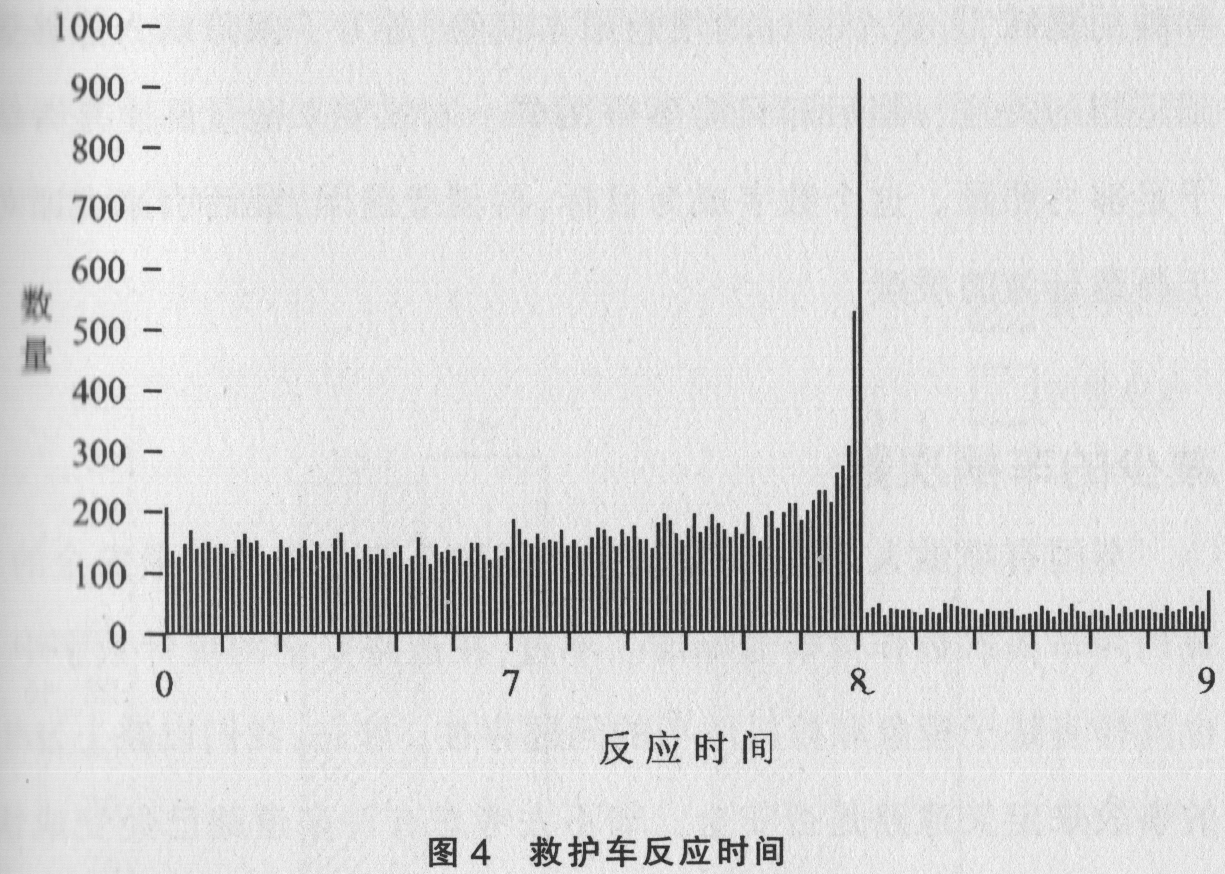
\includegraphics[width=0.55\textwidth]{c3.8min.01.png}
  \end{figure}
\end{frame}

\begin{frame}
  \frametitle{单一数字 | 案例 | 死亡35人}
  \begin{figure}
    \centering
    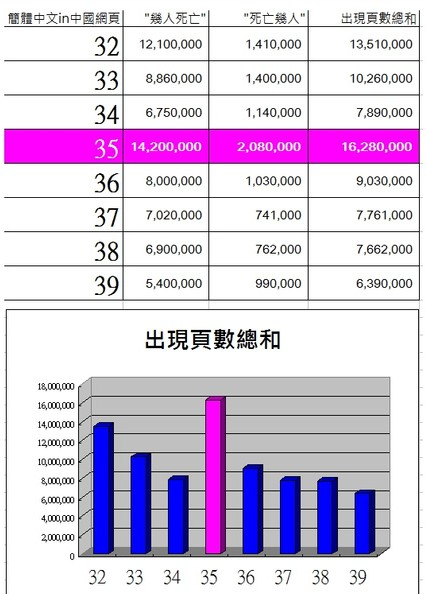
\includegraphics[width=0.45\textwidth]{c3.35.01.jpg}
  \end{figure}
\end{frame}

\begin{frame}
  \frametitle{单一数字 | 案例 | 车祸次数}
  \begin{block}{调查}
    2006年7月,《英国医学期刊》报道了一项关于车祸数据的调查,作者的结论是:在警方统计的数字中,非致命车祸伤员总数降低,“可能是因为汇报不完整”。
  \end{block}
  \begin{figure}
    \centering
    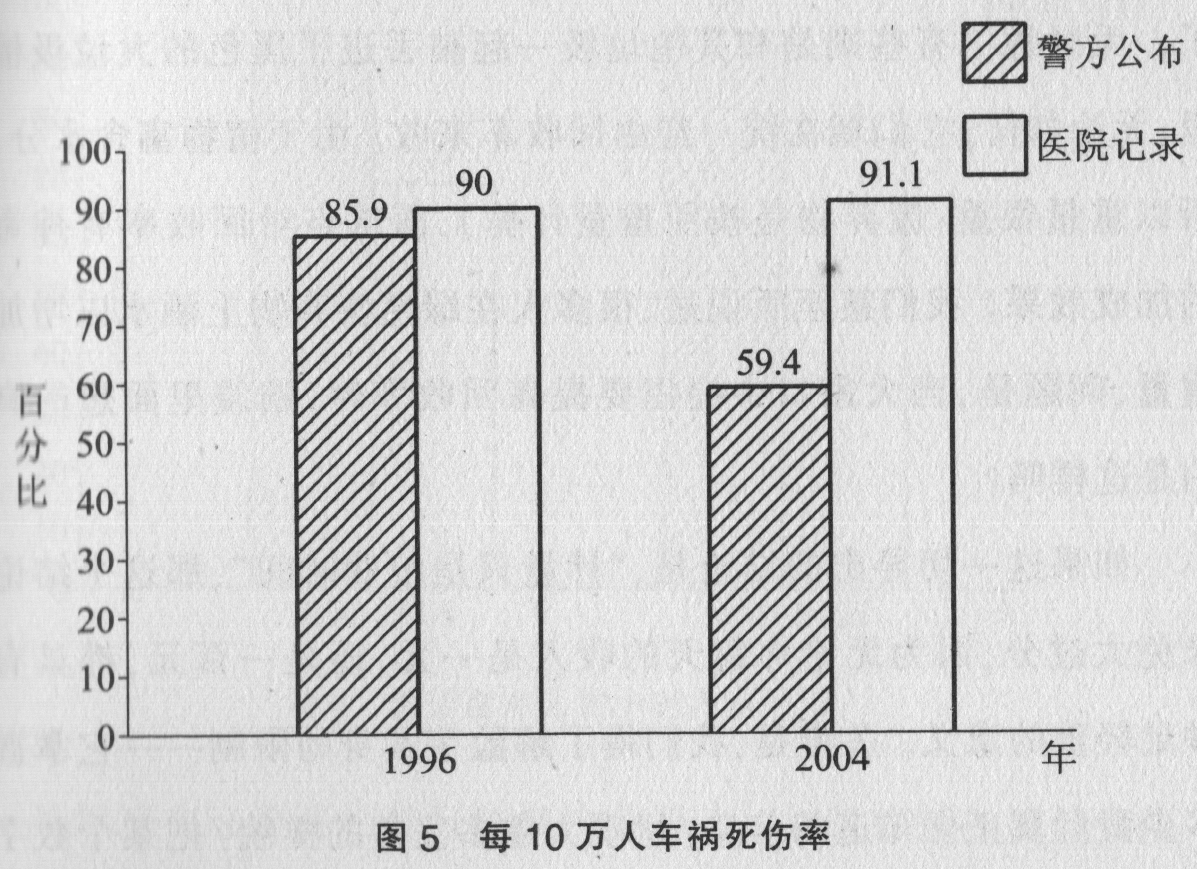
\includegraphics[width=0.6\textwidth]{c3.death.01.png}
  \end{figure}
\end{frame}

\begin{frame}
  \frametitle{单一数字 | 案例 | 有关顾客体验的绩效数据}
  \begin{figure}
    \centering
    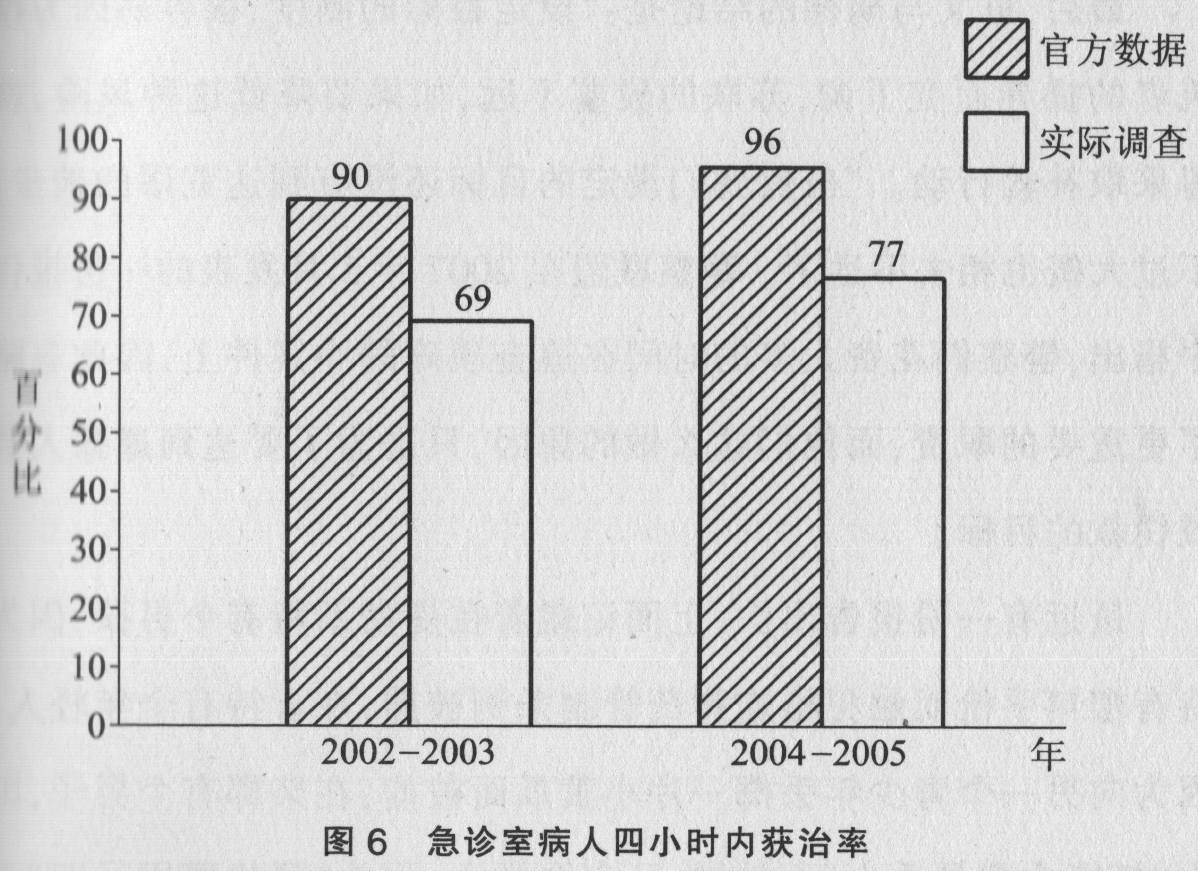
\includegraphics[width=0.8\textwidth]{c3.care.01.png}
  \end{figure}
\end{frame}

\begin{frame}
  \frametitle{单一数字 | 案例 | 预测孩子身高}
  \begin{block}{报道}
    “预测孩子长大后的身高,只需要利用现有的身高,再查表(一张适用于男孩,一张适用于女孩)中的比例(每个年龄段孩子的身高与最终身高的比例)即可”。
  \end{block}
  \pause \pause \pause \pause
  \begin{block}{解析}
    \begin{itemize}
      \item 所有孩子的生长方式并不是完全一致的:有的一开始长得很慢,却突然长高;有的暂时很高,然后速度趋缓;还有的人在整个过程中相对平稳地成长。
      \item 两张表是基于进行了大量测量之后所取的平均数。对于随机抽取的100名年轻人,利用这两张表格预测他们未来的总身高或者平均身高,毫无疑问是足够准确的。
      \item 但是,家长感兴趣的只是一个孩子的具体高度,对于个体,这两张表是没有价值的。
    \end{itemize}
  \end{block}
\end{frame}

\begin{frame}
  \frametitle{单一数字 | 案例 | 住房建设}
  \begin{block}{报道}
    原民主德国官方的统计数据一年又一年地庆祝住房建设的新纪录。
  \end{block}
  \pause \pause \pause \pause
  \begin{block}{解析}
    一套住房是什么?这些新“住房”中的许多住房却是养老院的房子或是重新修缮的老住宅。
  \end{block}
\end{frame}

\begin{frame}
  \frametitle{单一数字 | 案例 | 土著居民}
  \begin{block}{报道}
    加拿大“土著居民”的数量变得越来越多;自从5年前的一次人口统计以来,土著居民的人口数量几乎翻了一番。
  \end{block}
  \pause \pause \pause \pause
  \begin{block}{解析}
    这不是因为土著居民的数量实际增加了,而是因为越来越多的加拿大人被视为土著居民。
  \end{block}
\end{frame}

\begin{frame}
  \frametitle{单一数字 | 案例 | 疾病}
  \begin{block}{报道}
    \begin{itemize}
      \item 在美国与西班牙交战期间,美国海军的死亡率是0.9\%,而同时期纽约市居民的死亡率是1.6\%。这证明参军更安全。
      \item “去年是美国医学史上的小儿麻痹症年”。(癌症年,艾滋病年,肺结核年……)
    \end{itemize}
  \end{block}
  \pause \pause \pause \pause
  \begin{block}{解析}
    \begin{itemize}
      \item 海军主要由那些体格健壮的年轻人组成,而城市居民包括了婴儿、老人、病人,他们无论在哪儿死亡率都比较高。
      \item 当年有更多处于易感染期的孩子,认识加深、更频繁地到医院就诊、增加了轻微发病的记录,经济刺激、更多的小儿麻痹症保险和慈善机构更多的帮助。
    \end{itemize}
  \end{block}
\end{frame}

\begin{frame}
  \frametitle{单一数字 | 案例 | 疾病}
  \begin{block}{报道}
    \begin{itemize}
      \item 流感和肺炎几乎都出现在南方的3个州,它们占记录病例的80\%。
      \item 1940年以前,位于美国南部的一些地区一年内有成千上万例疟疾病例,而今天这些地区该病例减少到只有几例。这表明对于疟疾的治疗在短短几年中发生了有益且巨大的进步。
    \end{itemize}
  \end{block}
  \vspace{-0.4em}
  \pause \pause \pause \pause
  \begin{block}{解析}
    \begin{itemize}
      \item 目前只有这3个州仍然保留着对此类疾病的记录,其他地区已废除了这一做法。
      \item 现在只有在确诊为疟疾后才进行记录,而在以前,疟疾是南方人用以表示感冒或者着凉的方言。
    \end{itemize}
  \end{block}
  \vspace{-0.4em}
  \pause
  \begin{block}{死亡 vs. 发病}
    在考虑某种疾病的发病情况时,使用死亡率或者死亡人数比发病人数要更合理——这仅仅是因为死亡报道和死亡记录的质量更高。
  \end{block}
\end{frame}

\section{知识拓展}
\subsection{辛普森悖论}
\begin{frame}
  \frametitle{辛普森悖论}
  \begin{block}{辛普森悖论}
当人们尝试探究两种变量(比如新生录取率与性别)是否具有相关性的时候,会分别对之进行分组研究。然而,在分组比较中都占优势的一方,在总评中有时反而是失势的一方。
  \end{block}
  \pause
  \begin{block}{警示}
    \begin{itemize}
      \item 简单的将分组数据相加汇总,是不能反映真实情况的。
      \item 必需清楚了解情况,以综合考虑是否存在造成此悖论的潜在因素。
      \item 为了避免辛普森悖论的出现,就需要斟酌各分组的权重,并乘以一定的系数去消除因分组数据基数差异而造成的影响。
    \end{itemize}
  \end{block}
\end{frame}

\begin{frame}
  \frametitle{辛普森悖论}
  \begin{figure}
    \centering
    \visible<1->{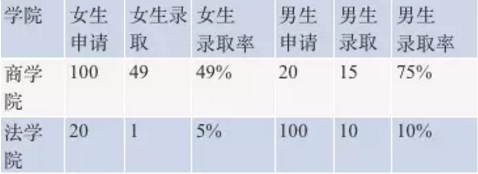
\includegraphics[width=0.5\textwidth]{c3.simpson.011.png}}\\
    \vspace{0.5em}
    \visible<2->{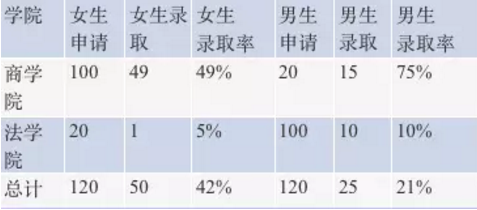
\includegraphics[width=0.5\textwidth]{c3.simpson.012.png}}\\
    \vspace{0.5em}
    \visible<3->{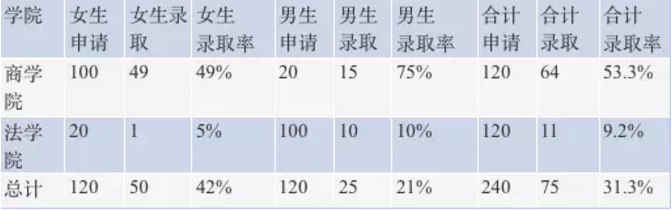
\includegraphics[width=0.5\textwidth]{c3.simpson.01.png}}
  \end{figure}
\end{frame}

\begin{frame}
  \frametitle{辛普森悖论}
  \begin{figure}
    \centering
    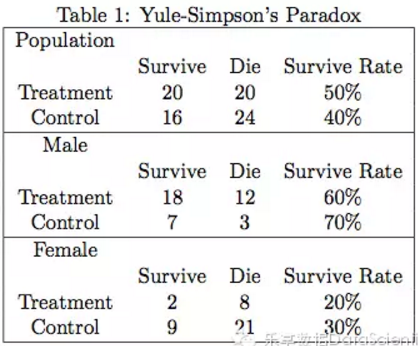
\includegraphics[width=0.7\textwidth]{c3.simpson.03.png}
  \end{figure}
\end{frame}

\subsection{区群谬误}
\begin{frame}
  \frametitle{区群谬误}
  \begin{block}{区群谬误}
    区群谬误(Ecological fallacy),又称生态谬误、层次谬误,是一种在分析统计资料时常犯的错误。和以偏概全相反,区群谬误是一种以全概偏,如果仅基于群体的统计数据就对其下属的个体性质作出推论,就是犯了区群谬误。这谬误假设了群体中的所有个体都有群体的性质(因此塑型(Sterotypes)也可能犯区群谬误)。区群谬误的相反情况为化约主义(Reductionism)。
  \end{block}
  \pause
  \begin{block}{举例}
一项研究发现甲城市民的智商平均比乙城市民高,若因此认为在两个城市各自随机抽取一个市民,甲城那位市民的智商都会比乙城的那位高,便犯上了区群谬误。因为统计结果只是对两城的平均智商作比较,乙城个别市民智商可能比甲城的个别市民高;在极端情况下,两城之中智商最高的一位市民可能生活在乙城。
  \end{block}
\end{frame}

\begin{frame}
  \frametitle{区群谬误}
  \begin{block}{区群谬误}
在1930年美国人口普查结果中,Robinson分析了48个州的识字率以及新移民人口比例的关系。他发现两者之间的相关系数为0.53,即代表若一个州的新移民比率愈高,平均来说这个州的识字率便愈高。\\
\vspace{0.5em}
但当分析个体资料时,便发现相关系数是-0.11,即平均来说新移民比本地人的识字率低。\\
  \end{block}
  \pause \pause \pause \pause
  \begin{block}{解析}
出现这种看似矛盾的结果,其实是因为新移民都倾向在识字率较高的州定居。
  \end{block}
  \pause
  \begin{block}{警示}
Robinson因此提出在处理群体资料、或区群资料时,必须注意到资料对个体的适用性。这并非指任何以群体资料对个体性质作出的推论都是错误的,但在推论时必须注意群体资料会否把群体内的变异隐藏起来。
  \end{block}
\end{frame}

\begin{frame}
  \frametitle{区群谬误}
  \begin{block}{区群谬误}
假设甲城和乙城都各有相同人数的富人和穷人,富人都住在山上,而穷人都住在排放致癌物的工厂附近,故此在两个城市的穷人癌症发病率都比富人高很多倍。在甲城的都是高增值高污染工业,故此在甲城无论是富人和穷人的平均工资都比乙城高,但同时甲城穷人的癌症发病率也因此比乙城高。\\
\vspace{1em}
一位教授希望找出癌症的风险因素,他在国家统计刊物找到甲城和乙城的癌症发病率和工资中位数,发现工资中位数较高的甲城有更高的癌症发病率,得出高收入是癌症风险因素的结论。然而事实上,贫穷才是癌症的风险因素,区群谬误带来相反的结论。
  \end{block}
\end{frame}

\begin{frame}
  \frametitle{区群谬误}
  \begin{figure}
    \centering
    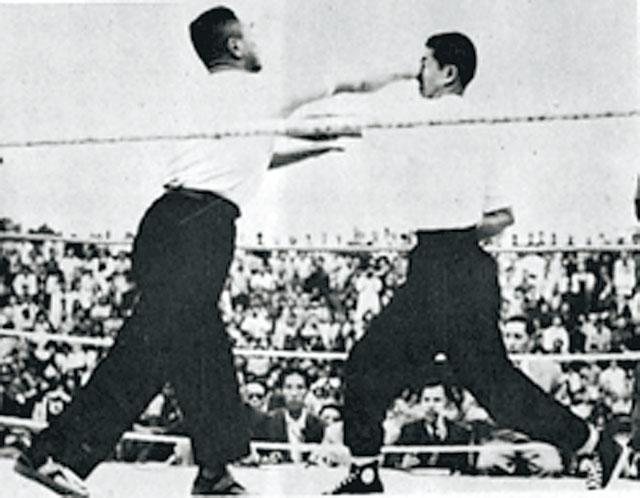
\includegraphics[width=0.45\textwidth]{c3.pk.01.jpg}\quad
    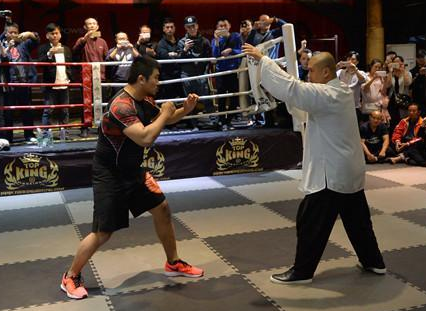
\includegraphics[width=0.48\textwidth]{c3.pk.02.png}
  \end{figure}
  \begin{block}{书籍}
    \begin{itemize}
      \item 徐皓峰:《逝去的武林》,《大成若缺》
    \end{itemize}
  \end{block}
\end{frame}

\subsection{生日问题}
\begin{frame}
  \frametitle{生日问题}
  \begin{block}{生日问题}
生日问题是指,如果一个房间里有23个或23个以上的人,那么至少有两个人的生日相同的概率要大于50\%。这就意味着在一个典型的标准小学班级(30人)中,存在两人生日相同的可能性更高。对于60或者更多的人,这种概率要大于99\%。\\
\vspace{0.3em}
从引起逻辑矛盾的角度来说生日悖论并不是一种悖论,从这个数学事实与一般直觉相抵触的意义上,它才称得上是一个悖论。大多数人会认为,23人中有2人生日相同的概率应该远远小于50\%。
  \end{block}
  \pause
  \begin{block}{比较}
    \begin{itemize}
      \item 至少有一个人的生日和张三的生日相同
      \item 至少有两个人的生日相同
    \end{itemize}
  \end{block}
\end{frame}

\begin{frame}
  \frametitle{生日问题}
  \begin{figure}
    \centering
    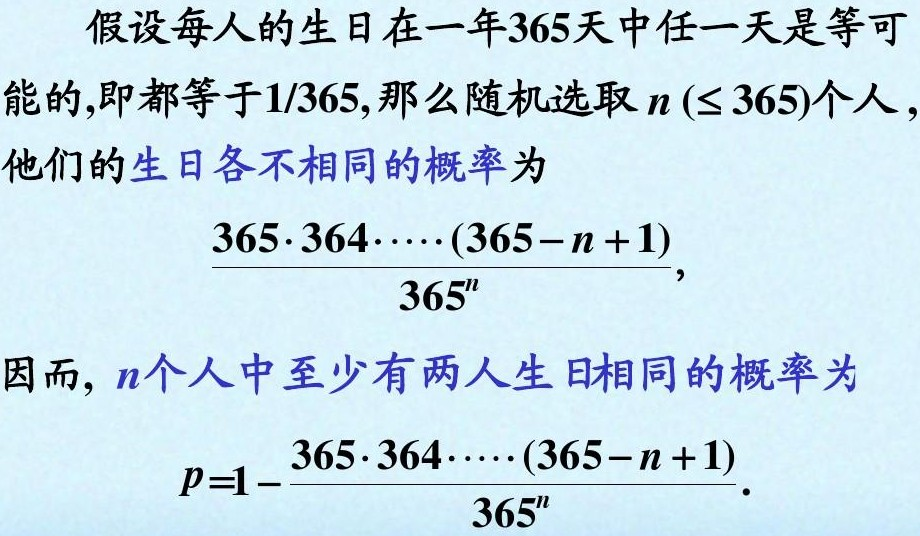
\includegraphics[width=0.9\textwidth]{c3.birthday.01.jpg}
  \end{figure}
\end{frame}

\begin{frame}
  \frametitle{生日问题}
  \begin{figure}
    \centering
    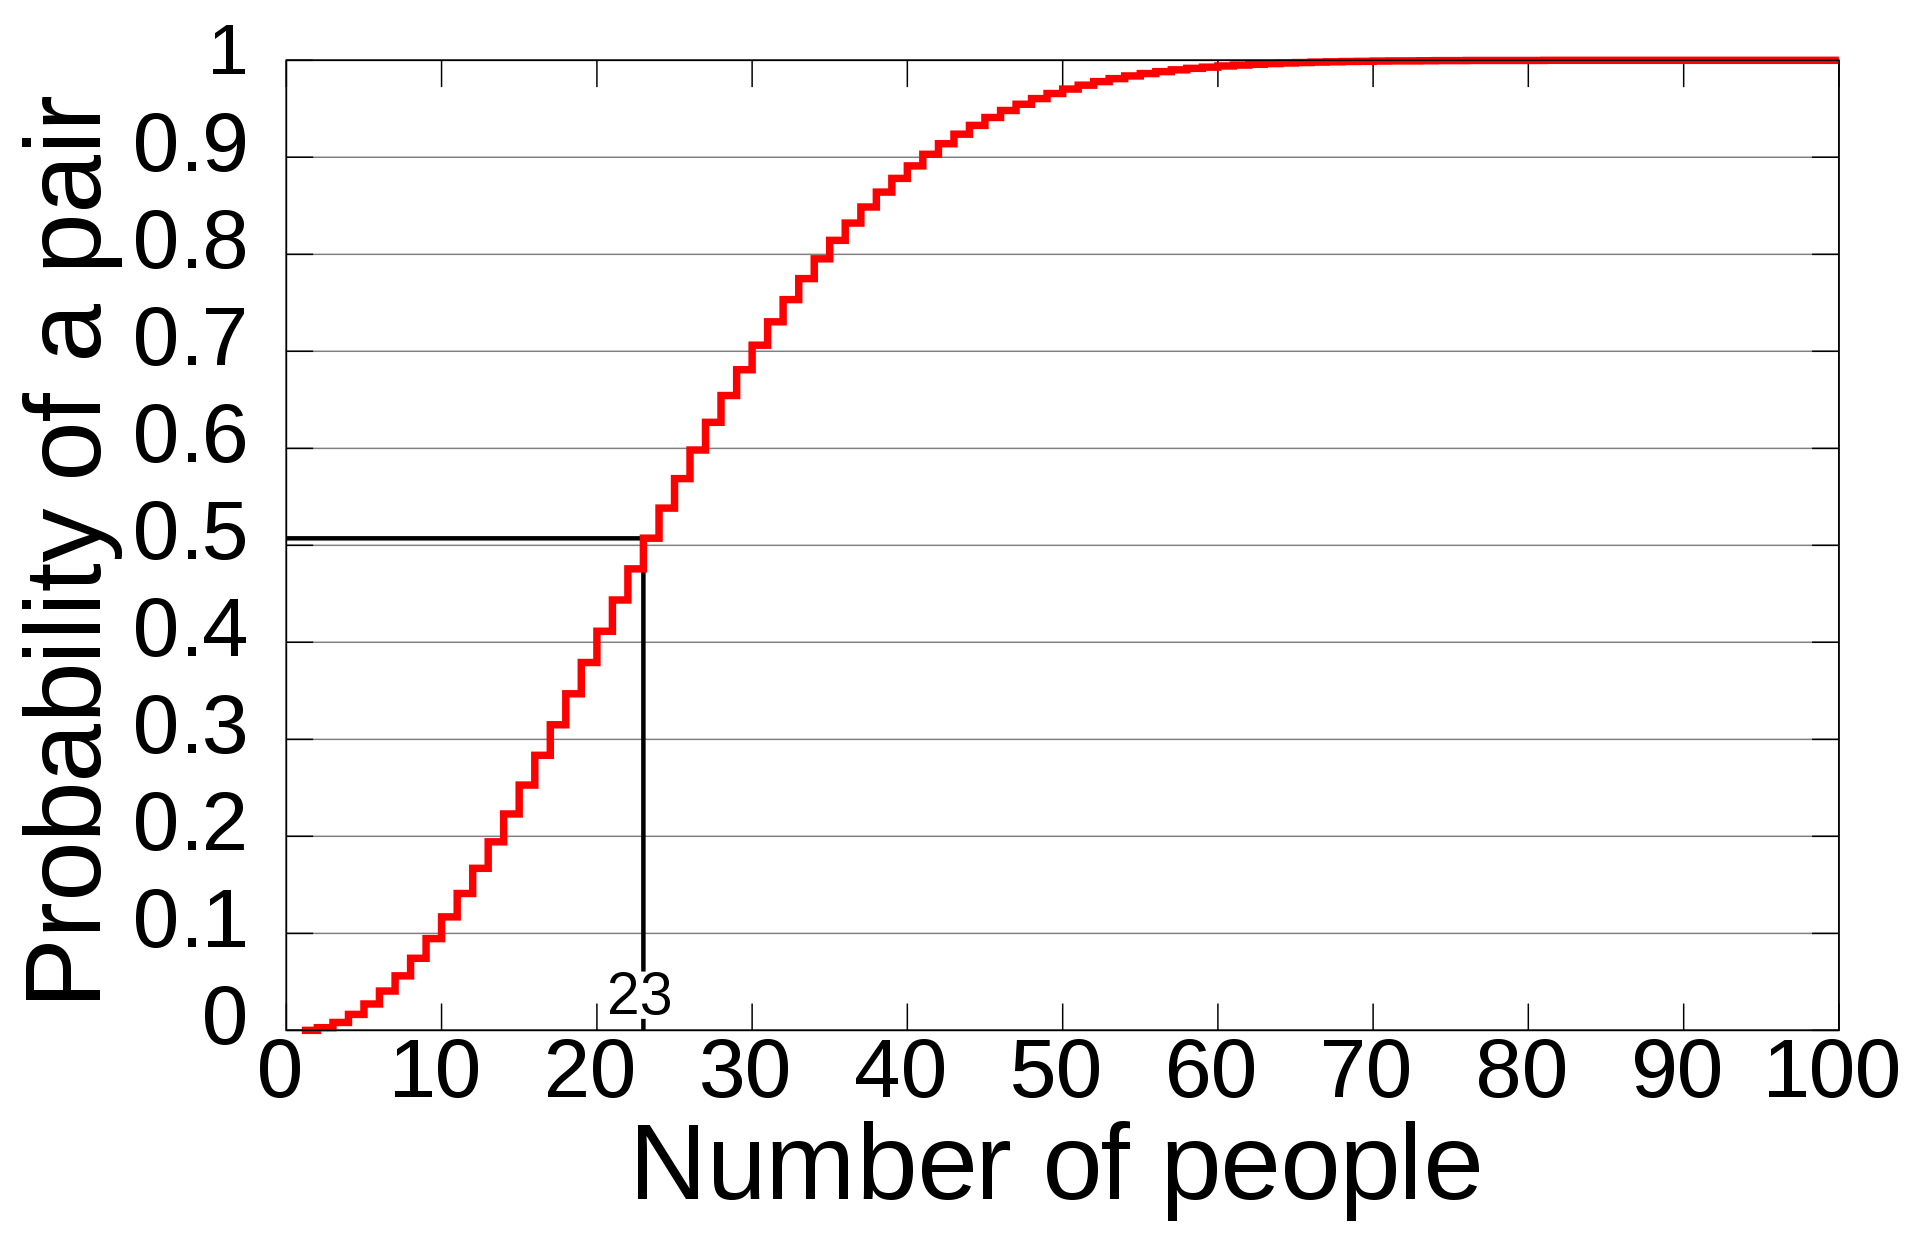
\includegraphics[width=0.5\textwidth]{c3.birthday.03.png}\\
    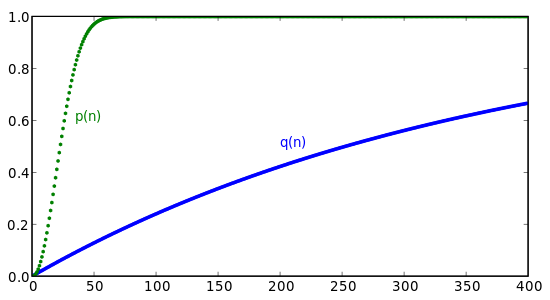
\includegraphics[width=0.5\textwidth]{c3.birthday.04.png}
  \end{figure}
\end{frame}

\subsection{鸽巢原理}
\begin{frame}
  \frametitle{鸽巢原理}
  \begin{block}{鸽巢原理(狄利克雷抽屉原理、鸽笼原理)}
    \begin{itemize}
      \item 若有n个笼子和n+1只鸽子,所有的鸽子都被关在鸽笼里,那么至少有一个笼子有至少2只鸽子。
      \item 若有n个笼子和kn+1只鸽子,所有的鸽子都被关在鸽笼里,那么至少有一个笼子有至少k+1只鸽子。
    \end{itemize}
  \end{block}
  \vspace{-0.5em}
  \begin{figure}
    \centering
    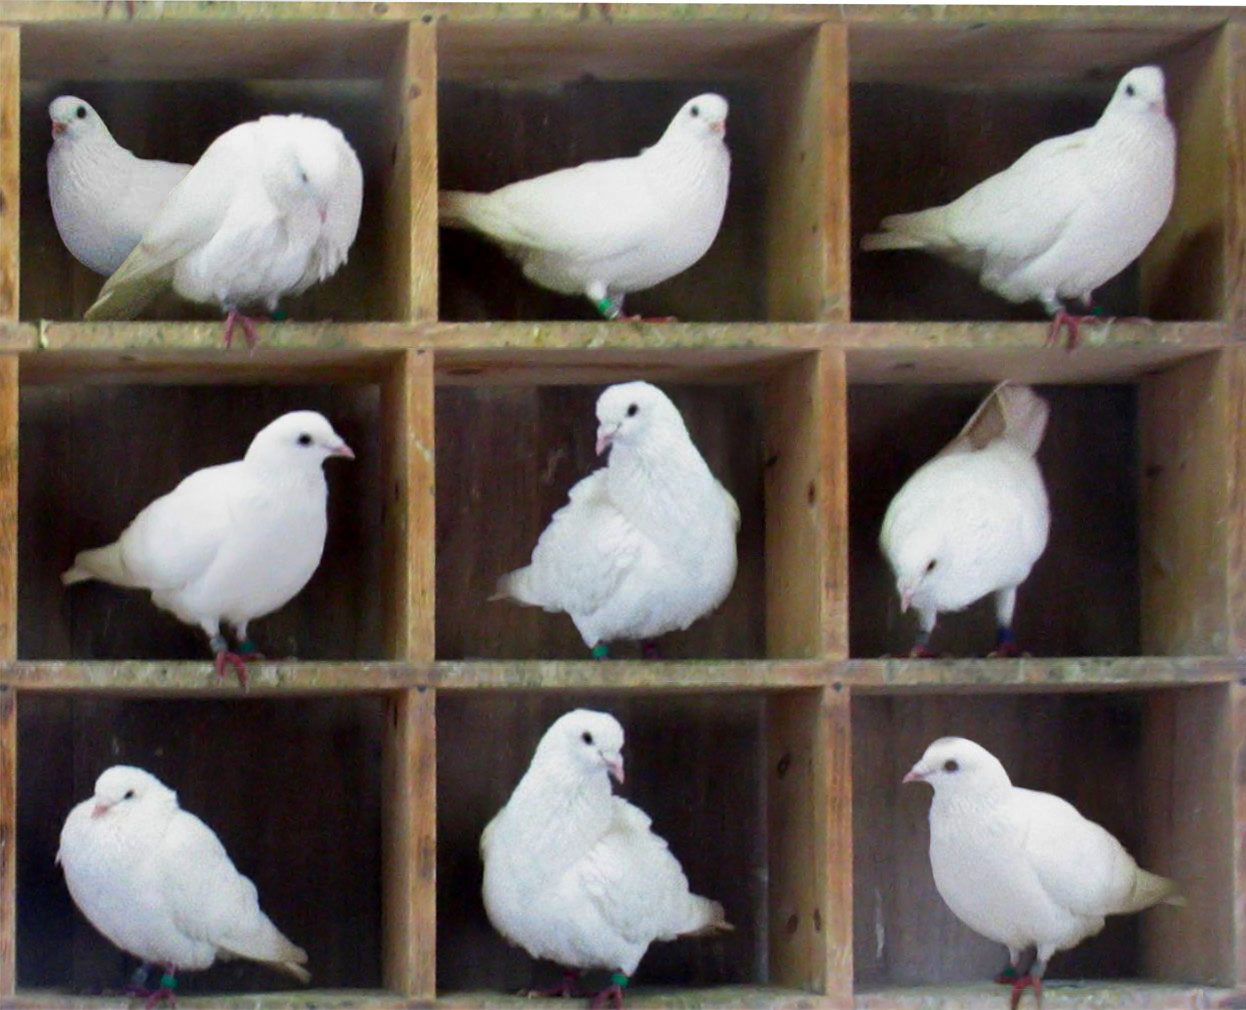
\includegraphics[width=0.45\textwidth]{c3.box.01.jpg}
  \end{figure}
\end{frame}

\begin{frame}
  \frametitle{鸽巢原理}
  \begin{block}{举例}
    \begin{itemize}
      \item 北京至少有两个人头发数一样多。
      \item 盒子里有10只黑袜子、12只蓝袜子,你需要拿一对同色的出来。假设你总共只能拿一次,需要拿几只?
    \end{itemize}
  \end{block}
  \pause \pause \pause \pause
  \begin{block}{解析}
    \begin{itemize}
      \item 常人的头发数在15万左右,可以假定没有人有超过100万根头发,但北京人口大于100万。如果我们让每一个鸽巢对应一个头发数字,鸽子对应于人,那就变成了有大于100万只鸽子要进到至多100万个巢中。所以,可以得到“北京至少有两个人头发数一样多”的结论。
      \item 只要3只就无法回避会拿到至少两只相同颜色的袜子,因为颜色只有两种(鸽巢只有两个),而有三只袜子(三只鸽子),从而得到“拿3只袜子出来,就能保证有一双同色”的结论。
    \end{itemize}
  \end{block}
\end{frame}

\begin{frame}
  \frametitle{课后阅读}
  \begin{block}{扩展链接}
    \begin{itemize}
      \item \href{http://www.thepaper.cn/newsDetail_forward_1500302}{破解神逻辑:不讲道理的人怎么总有理}
      \item \href{https://wx.abbao.cn/a/5248-c37c59ef8e0cd008.html}{中国人常犯的24个逻辑错误}
      \item \href{http://www.edu0-6.com/zixunzhuanqu/xingyedongtai/2216.html}{国外教育:这些逻辑谬误孩子从小被要求会辨识}
    \end{itemize}
  \end{block}
\end{frame}

\section{图说天下}
\subsection{蒙提霍尔问题}
\begin{frame}
  \frametitle{蒙提霍尔问题}
  \begin{figure}
    \centering
    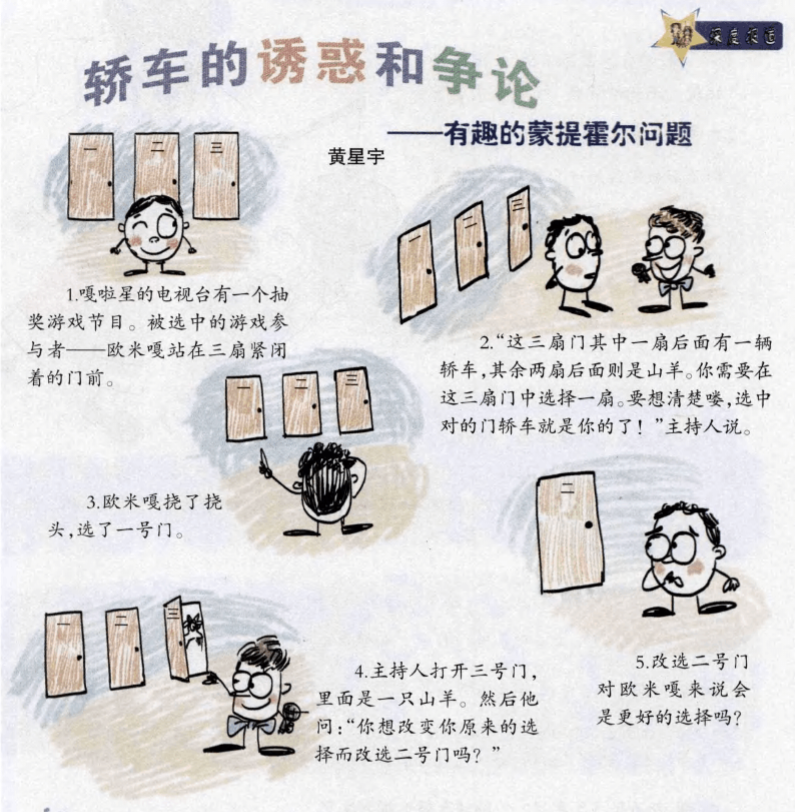
\includegraphics[width=0.6\textwidth]{c3.car.01.png}
  \end{figure}
\end{frame}

\begin{frame}
  \frametitle{蒙提霍尔问题 | 解答}
  \begin{figure}
    \centering
    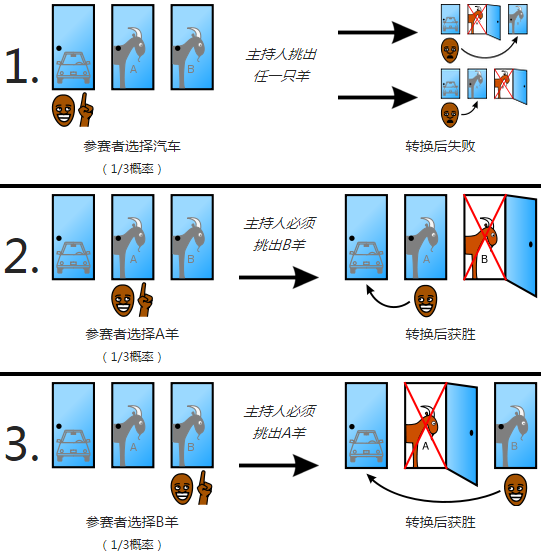
\includegraphics[width=0.6\textwidth]{c3.car.02.png}
  \end{figure}
\end{frame}
\begin{frame}
  \frametitle{蒙提霍尔问题 | 解答}
  \begin{figure}
    \centering
    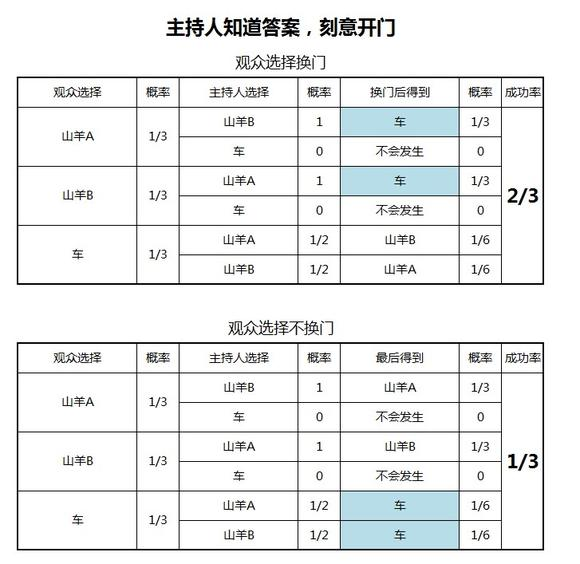
\includegraphics[width=0.6\textwidth]{c3.car.03.jpg}
  \end{figure}
\end{frame}


\section*{Acknowledgements}
\begin{frame}
  \frametitle{Powered by}
  \begin{center}
    
\includegraphics[width=9cm]{power.png}
  \end{center}
\end{frame}

\end{document}

